\chapter{Description de l'application mobile}\label{ch:app_mobile}

L'application mobile, aussi appelé RaceTracker dans ce document, permet de visualiser, en temps réel, les informations produites par les capteurs porté par les sportifs. En plus de cela elle permet également d'administrer les compétitions.

Elle est codée en langage Java et utilise le système Android et également le "Maps SDK for Android" de Google qui permet d'interagir avec les cartes ce qui permet l'ajout de marqueurs ou de dessiner des formes géométriques par exemple.

L'environnement de développement Android Studio a été utilisé pour le développement de cette application qui permet également de simuler l'exécution de l'application et facilite ainsi le débuggage.

\todo{Image GUI}

\section{Architecture logiciel}

L'architecture logiciel de l'application mobile est présentée ci-dessous. Une application Android est composée de "Activities", qui représentent chacun des écrans disponibles dans l'application. Des "Fragments" sont également utilisés, ce sont des morceaux d'interface graphique qui peuvent être insérés dans des "Activities". Enfin l'application mobile utilise des classes qui sont responsable de la gestion de l'application et de l'accès à la base de données.

La figure \ref{fig:app_static_archi} présente l'architecture statique de l'application mobile Android.

\begin{figure}[htb]
\centering 
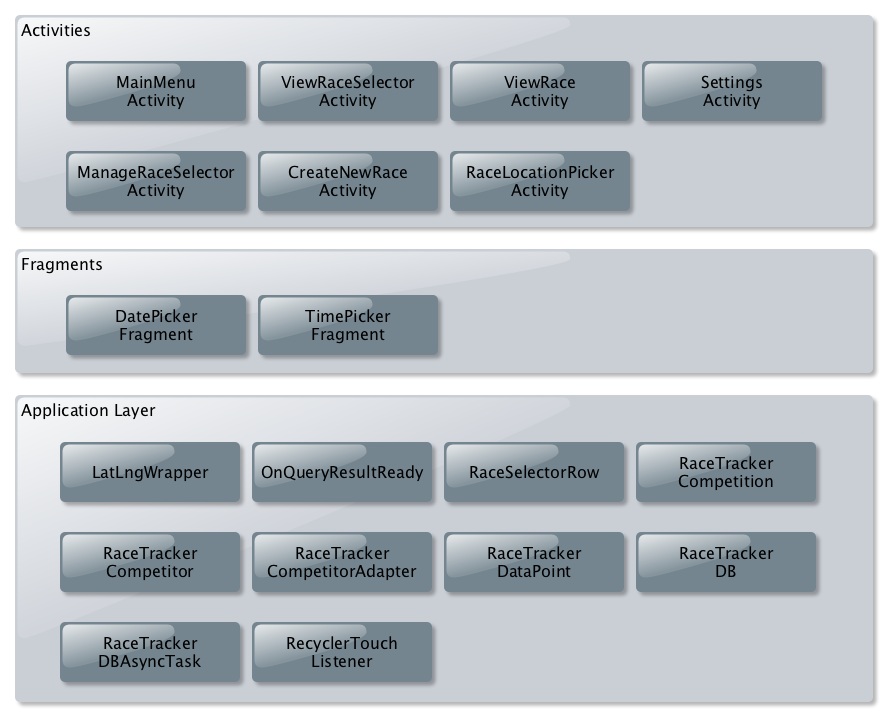
\includegraphics[width=1\columnwidth]{app_static_archi.png} 
\caption{Architecture statique de l'application mobile}
\label{fig:app_static_archi}
\end{figure}

Durant l'exécution de l'application mobile, le thread principal est entièrement géré par le système d'exploitation Android, il est en charge de la mise à jour de l'interface graphique et de tout ce qui est en lien comme par exemple le changement d'activité lors de l'appui d'un bouton. Lorsque l'application désire envoyer des requêtes à la base de données, elle utilise la classe RaceTrackerDBAsyncTask qui hérite de AsyncTask. Cette classe permet d'effectuer une tâche en arrière-plan de manière asynchrone et de gérer le résultat une fois la tâche terminée. Enfin, lorsque l'utilisateur est en train de visionner une course, un objet de type Handler est utilisé pour faire la requête du dernier point de donnée à intervalle régulier.

La figure \ref{fig:app_dyn_archi} montre l'architecture dynamique de l'application mobile. 

\begin{figure}[htb]
\centering 
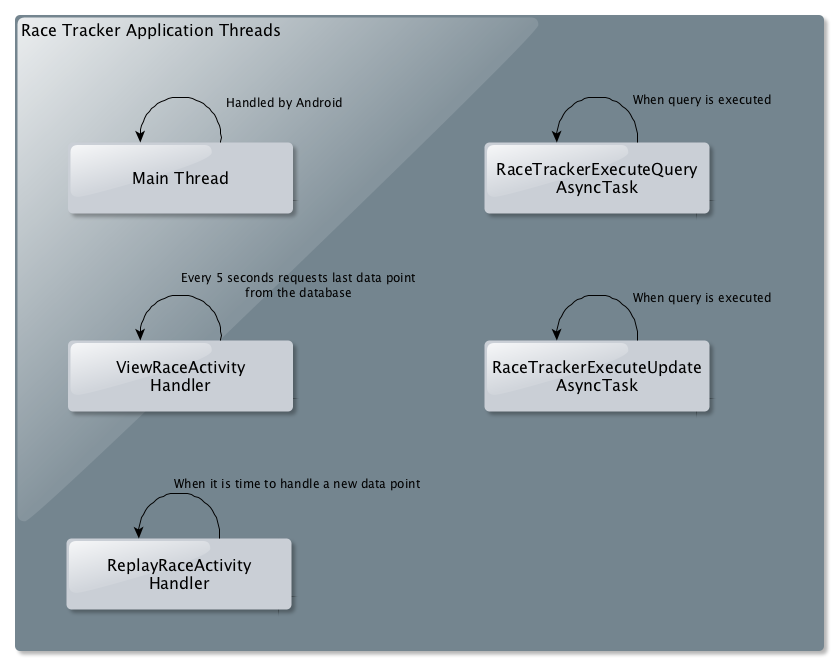
\includegraphics[width=1\columnwidth]{app_dyn_archi.png} 
\caption{Architecture dynamique de l'application mobile}
\label{fig:app_dyn_archi}
\end{figure}

\section{Les librairies externes}

L'application mobile utilise principalement deux librairies externes. La première est le "Maps for Android SDK”. Cette librairie permet d'ajouter à son application mobile une carte de type google maps et d'interagir avec elle. Elle permet d'ajouter des marqueurs à des positions (latitude/longitude) spécifiques, de créer des lignes entre les points ou encore de modifier le comportement de la carte. La librairie est disponible sur \url{https://cloud.google.com/maps-platform/}.

Un exemple d'utilisation est proposé ci-dessous.

\begin{lstlisting}[style=JavaStyle]
...
private GoogleMap mMap;

protected void onCreate(Bundle savedInstanceState) {
	/* Retrieve the map fragment when the map is ready */
	MapFragment mapFragment = (MapFragment) getFragmentManager().findFragmentById(R.id.mapView);
	mapFragment.getMapAsync(this);
}

@Override
public void onMapReady(GoogleMap googleMap) {
	mMap = googleMap;

	/* Change map type */
	mMap.setMapType(GoogleMap.MAP_TYPE_SATELLITE);

	/* Add a marker in Sydney, Australia */
	LatLng sydney = new LatLng(-34, 151);
	mMap.addMarker(new MarkerOptions().position(sydney).title("Marker in Sydney"));

	/* Move camera and zoom */
	mMap.moveCamera(CameraUpdateFactory.newLatLngZoom(sydney, -12));
}
...
\end{lstlisting}

La deuxième librairie externe utilisée est un driver de type JDBC permettant de s'interfacer avec une base de données PostgreSQL. C'est grâce à ce composant que l'application mobile va interroger la base de données afin de récupérer la liste des compétiteurs, les données relatives aux compétitions ou encore les points de données à afficher sur la carte. Le driver JDBC est téléchargeable gratuitement à l'adresse \url{https://jdbc.postgresql.org/}.

\begin{lstlisting}[style=JavaStyle]
...
public ResultSet executeQuery(String connection, String user, String password, String query) {
	Statement st;
	ResultSet results

	Connection conn = DriverManager.getConnection(connection, user, password);
	st = conn.createStatement();
	
	results = st.executeQuery(query);
	st.close()	
	
	return results;
}

public void myQuery() {
	String myQuery = "SELECT * FROM my_table;";
	ResultSet results;
	
	results = executeQuery("jdbc:postgresql://192.168.1.4:5432/mydatabase", "me", "1234", myQuery);
	
	while (results.getResult().next()) {
		System.out.println("Field test1: " + results.getString("field_test_1"));
		System.out.println("Field test2: " + results.getInt("field_test_2"));
	}
	
	results.close();	
}
...
\end{lstlisting}

\section{Accès à la base de données}

Les accès à la base de données sont fait de manière similaire peut importe la requête en elle même. La seule différenciation est entre les requêtes de type SELECT et les mise à jours des données (UPDATE, DELETE ou INSERT). Le comportement est un peu différent dans la mesure ou une requête de type SELECT attend en retour un résultat qui comporte les données demandées à la base. Dans le cas d'une mise à jour, seul le nombre d'élément dans la base est retourné.

Afin d'exécuter une requête l'on créera une instance d'une classe RaceTrackerQuery qui contient la requête en elle même ainsi que les fonctions de callback qui seront appelé au fil de l'évolution de l'exécution de la requête. La classe RaceTrackerQuery utilise les classes RaceTrackerExecuteQuery et RaceTrackerExecuteUpdate en fonction du type de requête. Ces deux objets utilisent le concept de ASyncTask afin d'exécuter les requête en arrière plan et ainsi ne pas bloquer le thread principale pendant trop de temps.

Afin de pouvoir récupérer les résultats d'une requête de type SELECT, les classes devront implémenter les interface OnQueryResultsReady et OnQueryExecuted. La première est appelé lorsque les résultats venant de la base de données sont prêt à être analyser. La deuxième interface est appelé lorsque l'exécution de la requête est terminés.

Si l'on désire exécuter une requête de mise à jour alors il faudra implémenter OnUpdateDone qui permettra, au terme de l'exécution de la requête, combien d'élément ont été modifier.

\section{Les activités}

Dans le monde Android, une activité est une chose singulière que l'utilisateur peut effectuer. La majorité des activités interagissent avec l'utilisateur au travers de l'interface graphique afin d'effectuer une certaine tâche. \cite{android-activity} Dans le cas de l'application développée dans le cadre du travail de diplôme les activités utilisées sont décrite ci-dessous.

\subsection{MainMenuActivity}

Le point d'entrée de l'application Android est le premier écran qui se lance, et qui permet de choisir si l'on souhaite visionner une course ou alors faire des opérations d'administration sur la base de données. Lorsque l'utilisateur a fait son choix, elle lance l'activité, suivante c'est à dire soit ViewRaceSelectorActivity ou ManageRaceSelectorActivity.

La figure \ref{fig:mainmenuactivity_uml} montre le diagramme de classe de MainMenuActivity.

\begin{figure}[htb!]
    \centering
    \begin{subfigure}[htb]{0.49\textwidth}
		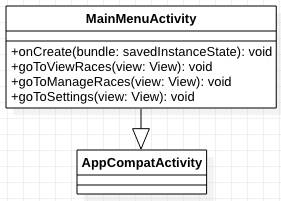
\includegraphics[width=1\columnwidth]{mainmenuactivity_uml.png} 
		\caption{Diagramme de classe}
		\label{fig:mainmenuactivity_uml}
    \end{subfigure}
    ~ %add desired spacing between images, e. g. ~, \quad, \qquad, \hfill etc. 
      %(or a blank line to force the subfigure onto a new line)
    \begin{subfigure}[htb]{0.49\textwidth}
		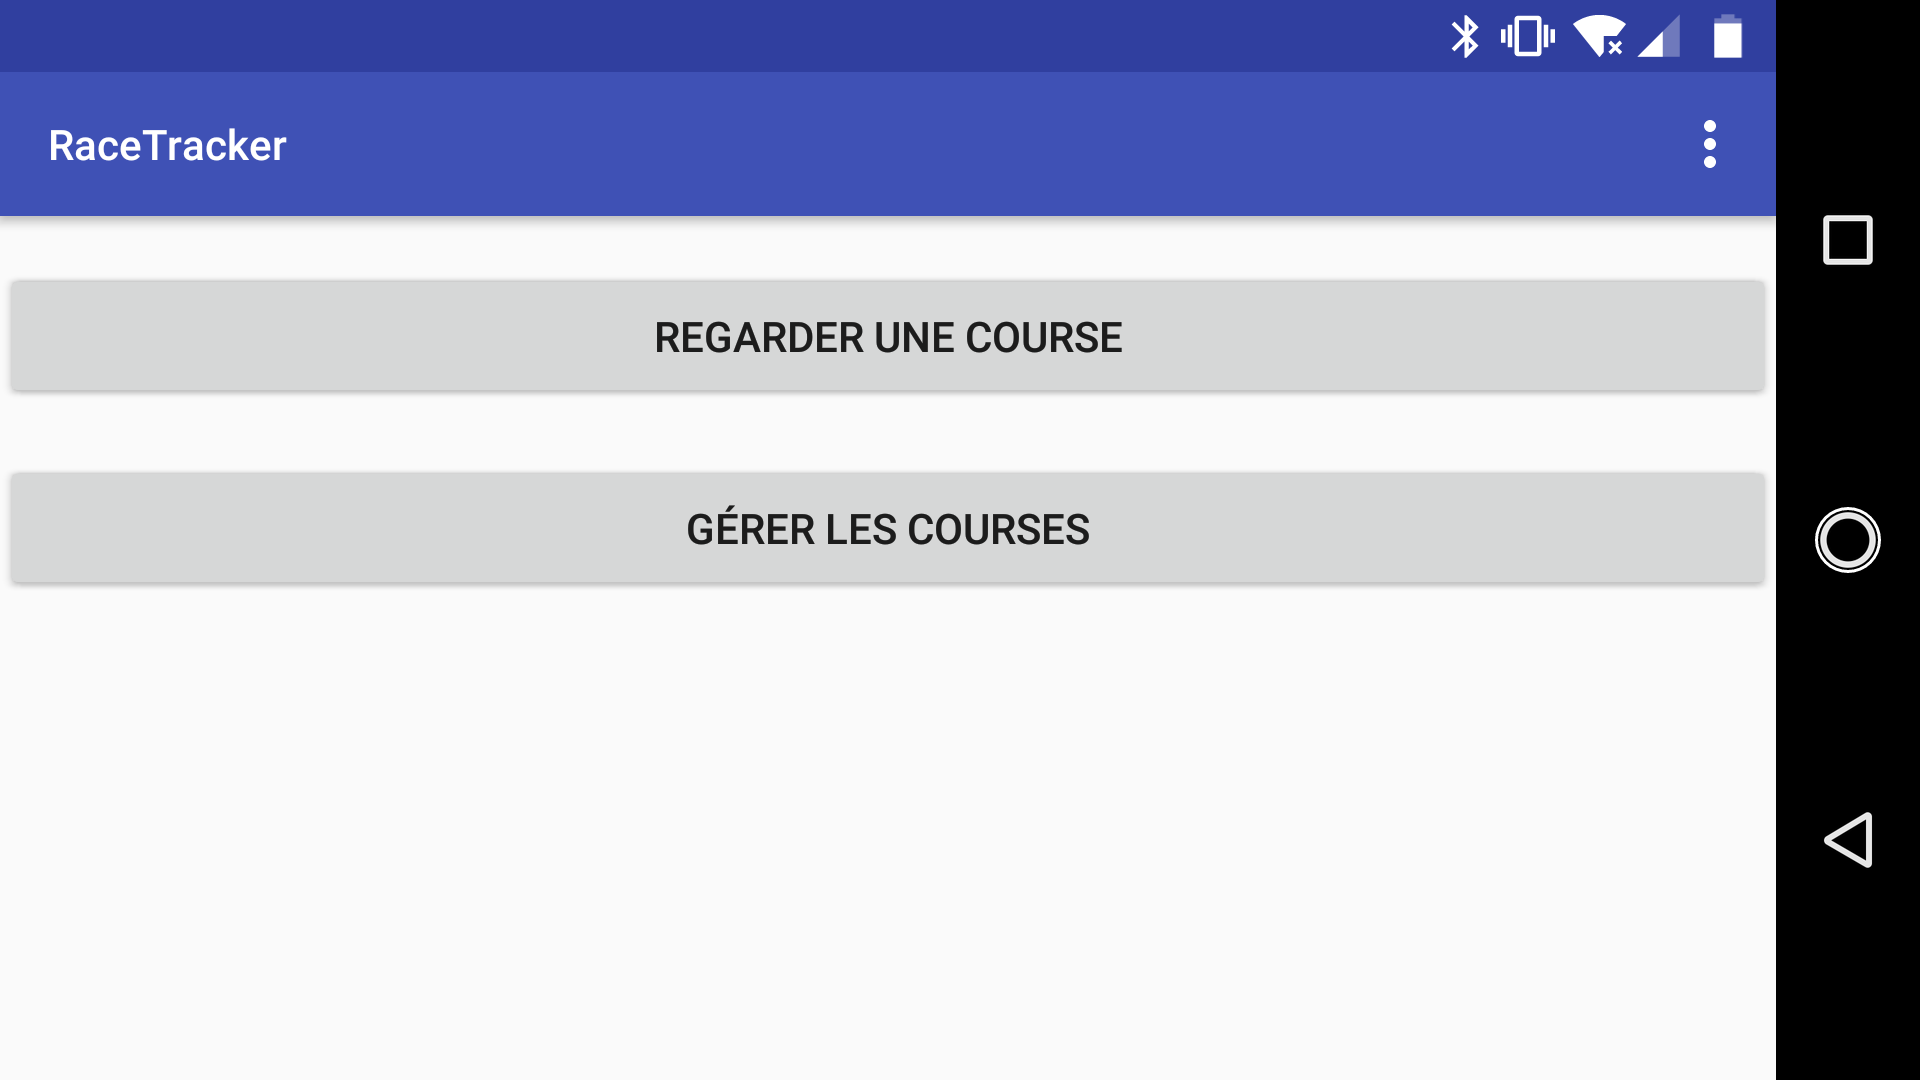
\includegraphics[width=1\columnwidth]{mainmenuactivity_gui.png} 
		\caption{Aperçu de l'interface graphique de l'activité}
		\label{fig:mainmenuactivity_gui}
    \end{subfigure}
    \caption{MainMenuActivity}\label{fig:mainmenuactivity_fig}
\end{figure}

\subsection{ViewRaceSelectorActivity}

Cette activité permet à l'utilisateur de sélectionner une course. Lorsqu'elle se lance, elle va aller interroger la base de données afin de récupérer la liste de toutes les compétitions et l'afficher à l'utilisateur qui peut ensuite sélectionner une course en cliquant sur l'objet de son choix. Une fois la course choisie, un objet de type RaceTrackerCompetition contenant les informations relatives à la course est renvoyé au créateur de cette activité.

La figure \ref{fig:viewraceselector_uml} montre le diagramme de classe de ViewRaceSelectorActivity.

\begin{figure}[htb!]
    \centering
    \begin{subfigure}[htb]{0.49\textwidth}
		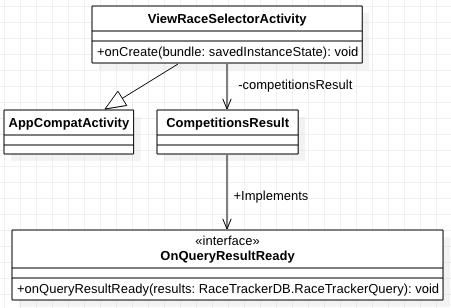
\includegraphics[width=1\columnwidth]{viewraceselector_uml.png} 
		\caption{Diagramme de classe}
		\label{fig:viewraceselector_uml}
    \end{subfigure}
    ~ %add desired spacing between images, e. g. ~, \quad, \qquad, \hfill etc. 
      %(or a blank line to force the subfigure onto a new line)
    \begin{subfigure}[htb]{0.49\textwidth}
		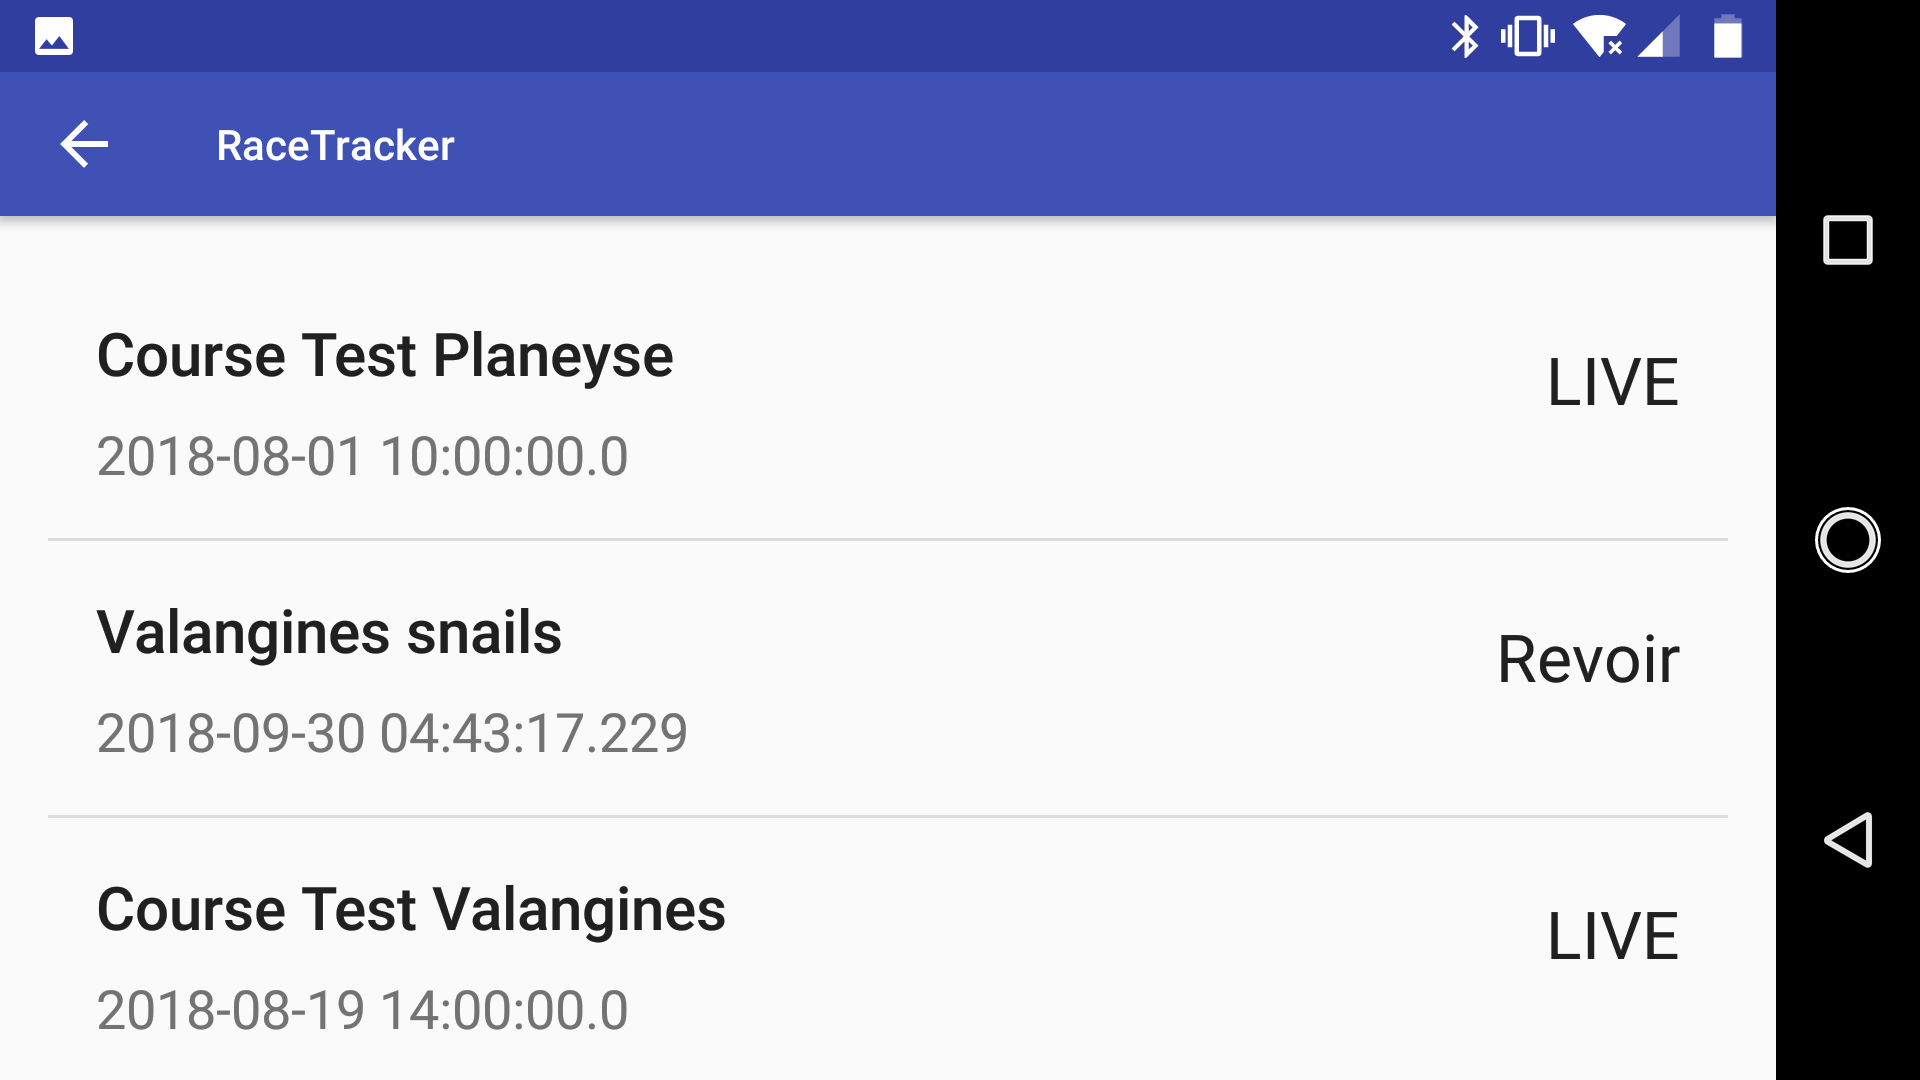
\includegraphics[width=1\columnwidth]{viewraceselector_gui.png} 
		\caption{Aperçu de l'interface graphique de l'activité}
		\label{fig:viewraceselector_gui}
    \end{subfigure}
    \caption{ViewRaceSelectorActivity}\label{fig:viewraceselector_fig}
\end{figure}

\subsection{ViewRaceActivity}

Lorsque l'utilisateur désire regarder une course, c'est cette activité qui va être lancée. Elle est responsable de la gestion de l'affichage des informations sur la carte et également de la liste des compétiteurs. Périodiquement cette activité va aller chercher dans la base de données les points de données relatifs à une course et vérifier si de nouveaux points ont été ajoutés, auquel cas elle met à jour la carte avec la nouvelle position. Toutes ces informations sont récupérées depuis la base de données.

La figure \ref{fig:viewraceactivity_uml} montre le diagramme de classe de ViewRaceActivity.

\begin{figure}[htb!]
    \centering
    \begin{subfigure}[htb]{0.49\textwidth}
		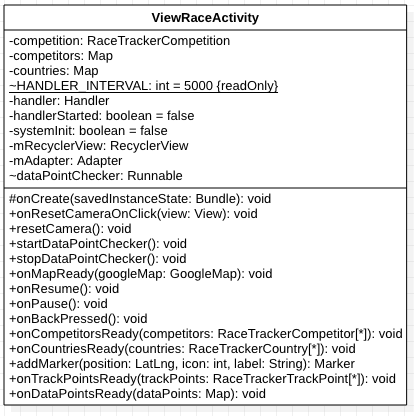
\includegraphics[width=1\columnwidth]{viewraceactivity_uml.png} 
		\caption{Diagramme de classe}
		\label{fig:viewraceactivity_uml}
    \end{subfigure}
    ~ %add desired spacing between images, e. g. ~, \quad, \qquad, \hfill etc. 
      %(or a blank line to force the subfigure onto a new line)
    \begin{subfigure}[htb]{0.49\textwidth}
		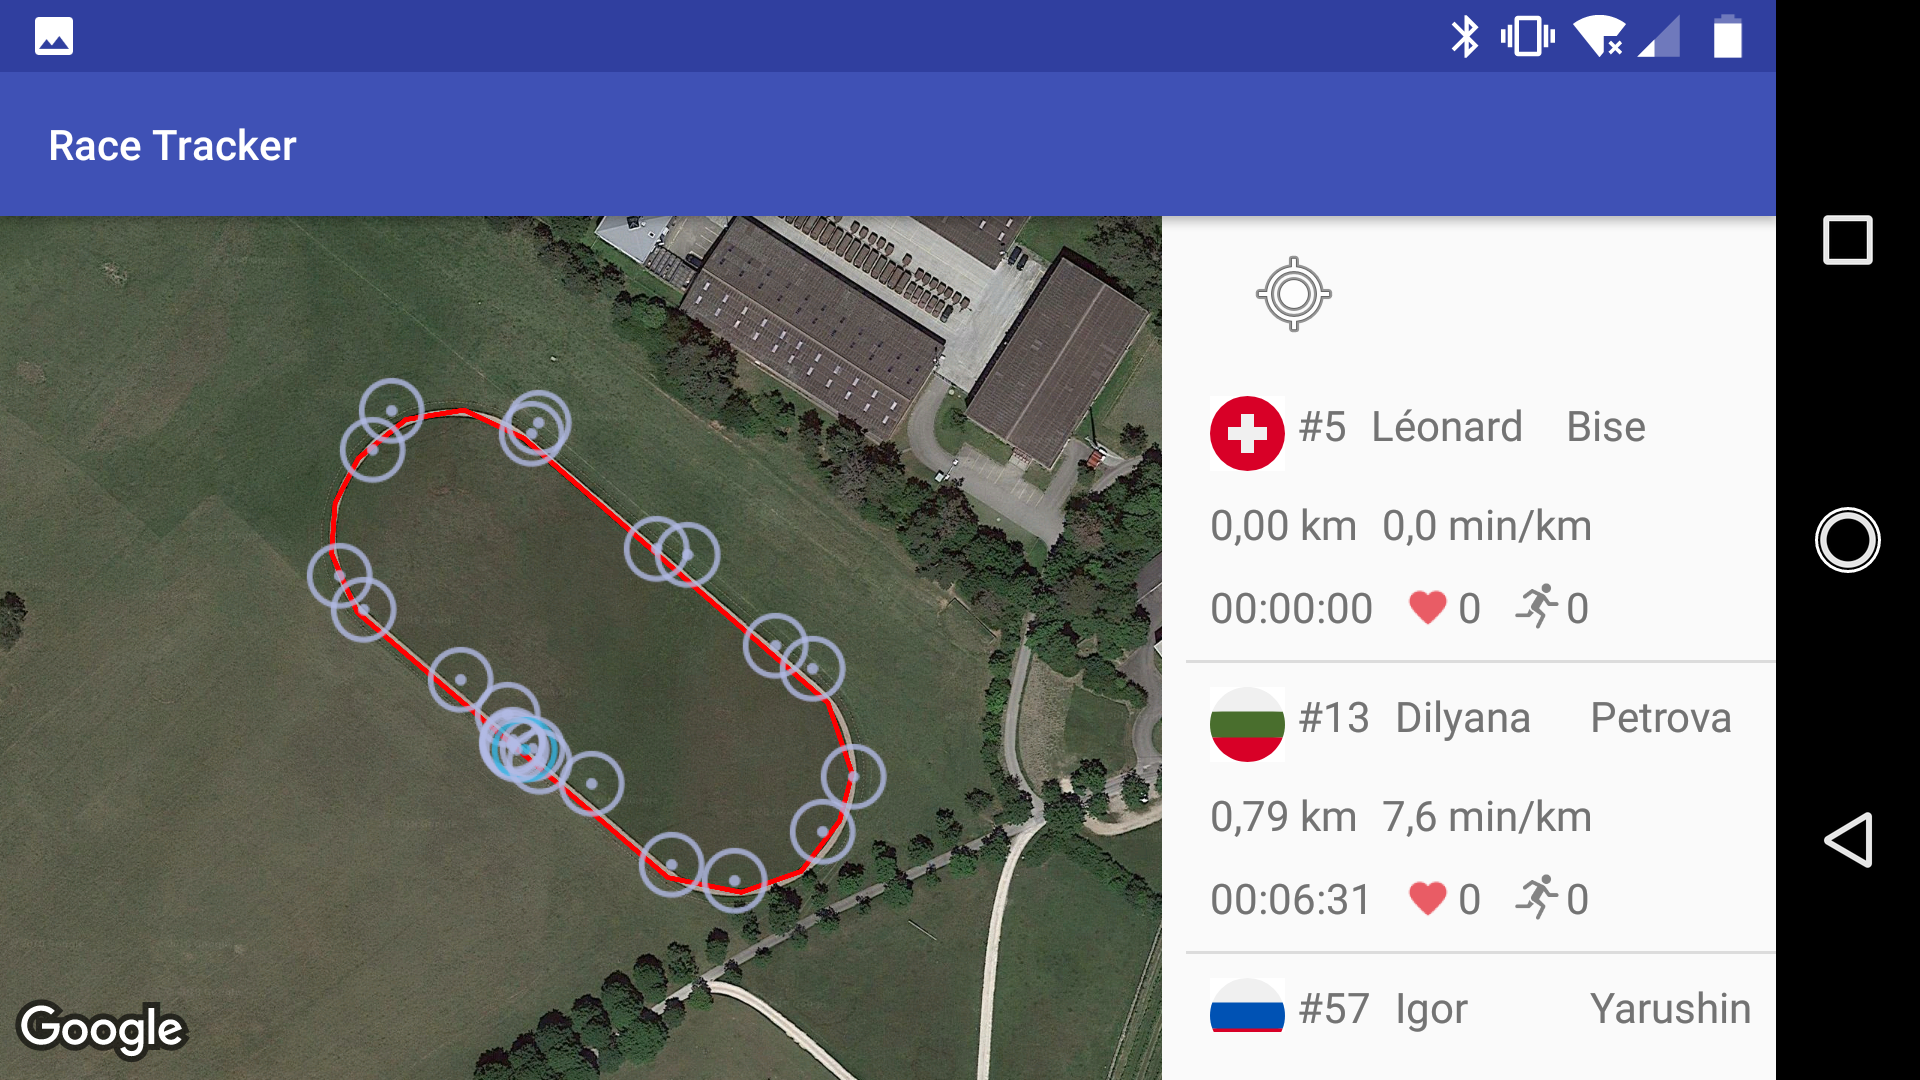
\includegraphics[width=1\columnwidth]{viewraceactivity_gui.png} 
		\caption{Aperçu de l'interface graphique de l'activité}
		\label{fig:viewraceactivity_gui}
    \end{subfigure}
    \caption{ViewRaceActivity}\label{fig:viewraceactivity_fig}
\end{figure}

\subsection{ReplayRaceActivity}

L'activité ReplayRaceActivity est très semblable et donc hérite de ViewRaceActivity. Son but est d'afficher une course déjà terminée et donc de reconstituer la course comme lorsqu'elle s'est passée. Elle va récupérer tous les points de données puis calculer le temps qui est passé entre chacun d'eux afin de pouvoir simuler l'évolution de la course comme en direct.

La figure \ref{fig:replayrace_uml} montre le diagramme de classe de ReplayRaceActivity.

\begin{figure}[htb!]
    \centering
    \begin{subfigure}[htb]{0.49\textwidth}
		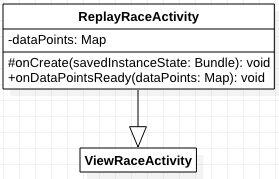
\includegraphics[width=1\columnwidth]{replayrace_uml.png} 
		\caption{Diagramme de classe}
		\label{fig:replayrace_uml}
    \end{subfigure}
    ~ %add desired spacing between images, e. g. ~, \quad, \qquad, \hfill etc. 
      %(or a blank line to force the subfigure onto a new line)
    \begin{subfigure}[htb]{0.49\textwidth}
		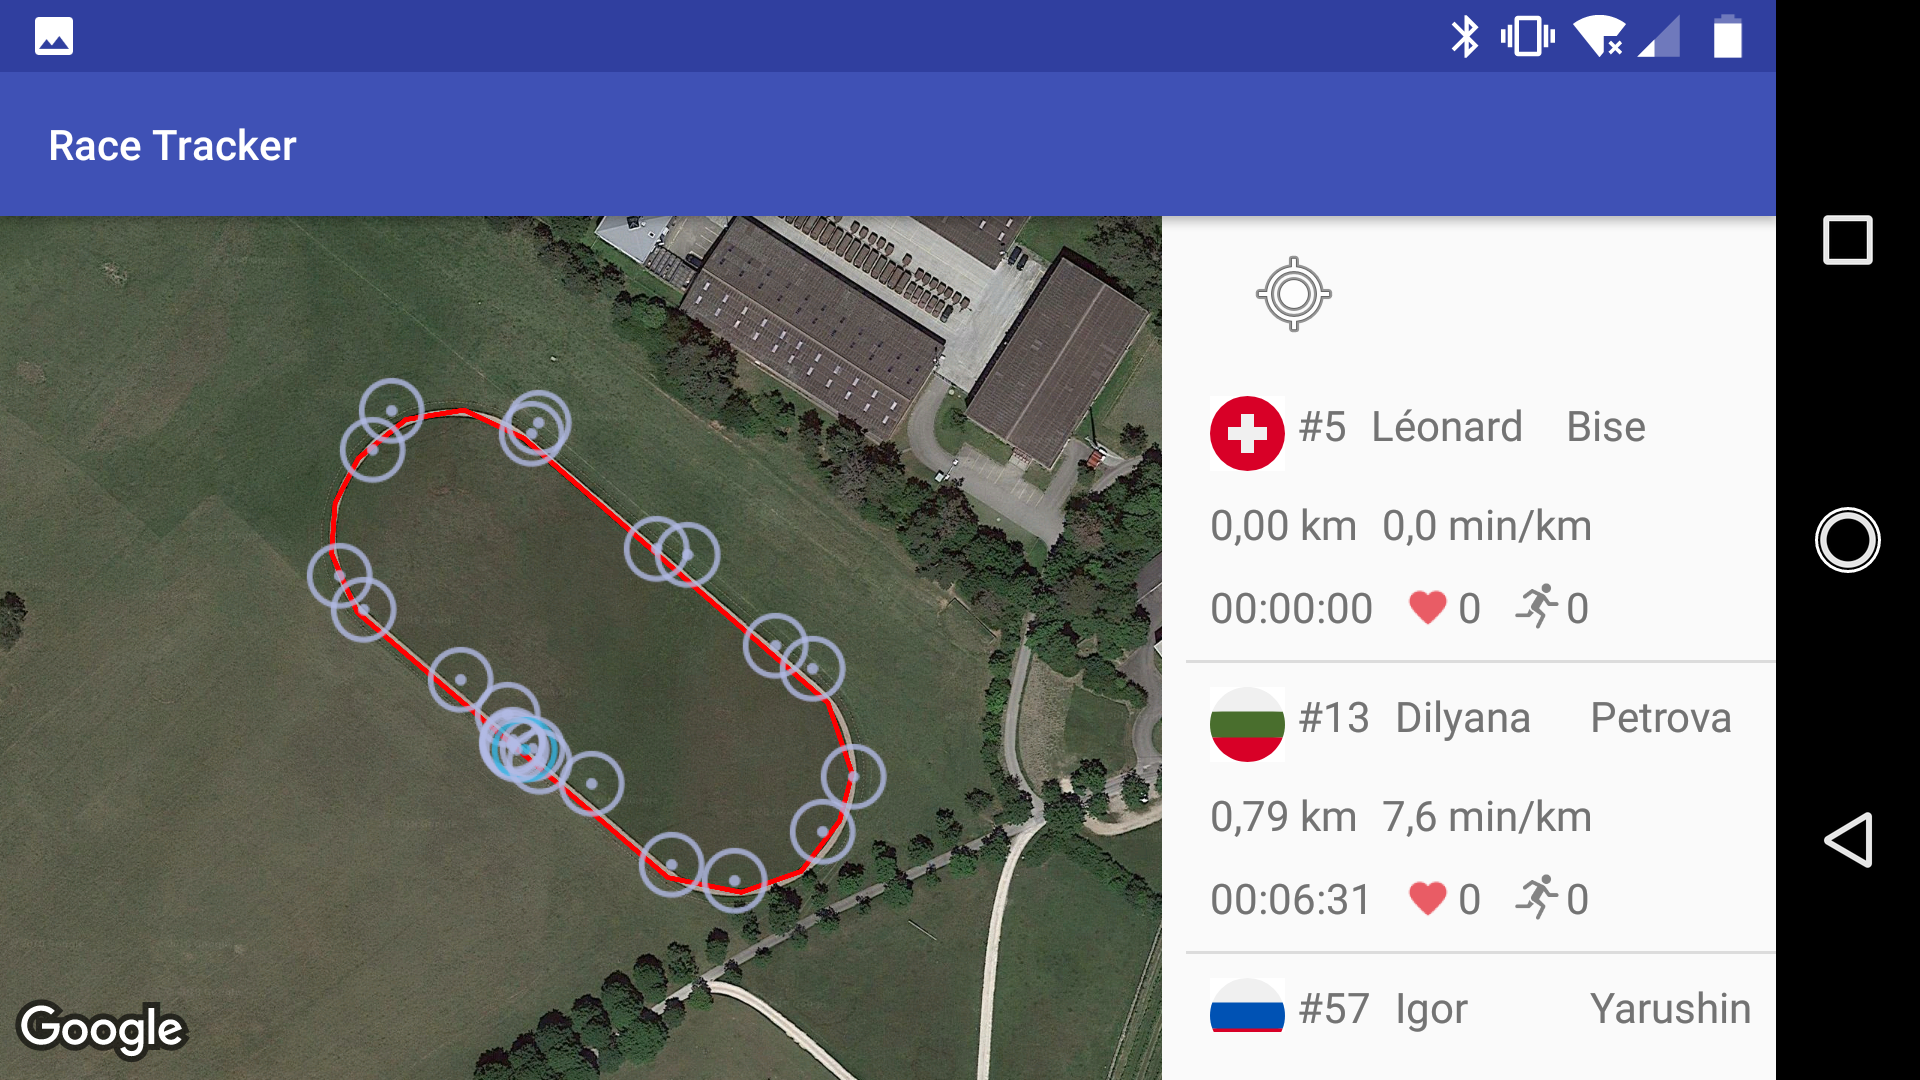
\includegraphics[width=1\columnwidth]{viewraceactivity_gui.png} 
		\caption{Aperçu de l'interface graphique de l'activité}
		\label{fig:replayrace_gui}
    \end{subfigure}
    \caption{ReplayRaceActivity}\label{fig:replayrace_fig}
\end{figure}

\todo{Maj GUI image}

\subsection{ManageRaceSelectorActivity}

La classe ManageRaceSelectorActivity permet à l'utilisateur de sélectionner l'action d'administration qu'il désire effectuer. Une fois la sélection  faite, l'activité correspondante est lancée.

La figure \ref{fig:manageraceselector_uml} montre le diagramme de classe de ManageRaceSelectorActivity.

\begin{figure}[htb!]
    \centering
    \begin{subfigure}[htb]{0.49\textwidth}
		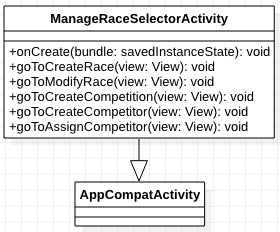
\includegraphics[width=1\columnwidth]{manageraceselector_uml.png} 
		\caption{Diagramme de classe}
		\label{fig:manageraceselector_uml}
    \end{subfigure}
    ~ %add desired spacing between images, e. g. ~, \quad, \qquad, \hfill etc. 
      %(or a blank line to force the subfigure onto a new line)
    \begin{subfigure}[htb]{0.49\textwidth}
		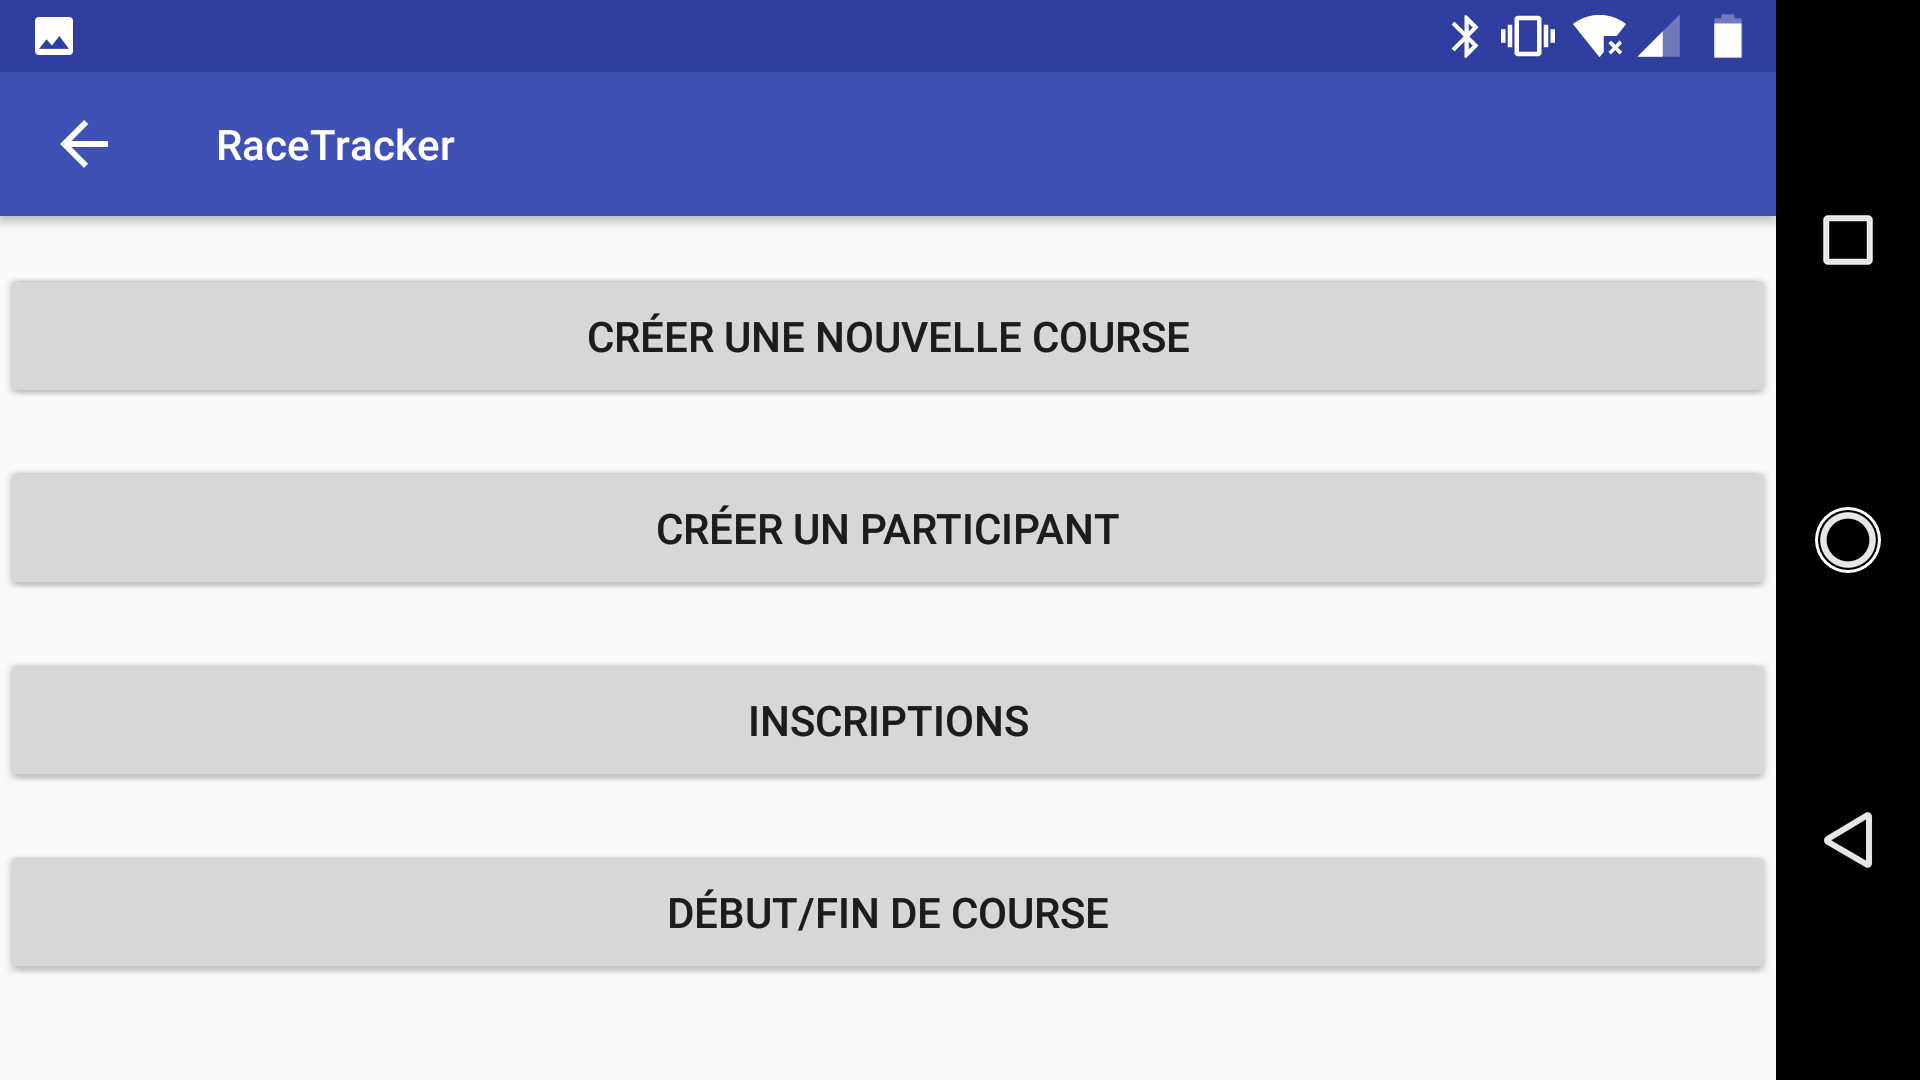
\includegraphics[width=1\columnwidth]{manageraceselector_gui.png} 
		\caption{Aperçu de l'interface graphique de l'activité}
		\label{fig:manageraceselector_gui}
    \end{subfigure}
    \caption{ViewRaceActivity}\label{fig:manageraceselector_fig}
\end{figure}

\subsection{CreateNewRaceActivity}

L'activité CreateNewRaceActivity permet à l'utilisateur de créer une nouvelle compétition dans la base de données. Une fois que l'utilisateur a rentré toutes les informations, une requête d'insertion est envoyée à la base de données.

La figure \ref{fig:createnewrace_uml} montre le diagramme de classe de CreateNewRaceActivity.

\begin{figure}[htb!]
    \centering
    \begin{subfigure}[htb]{0.49\textwidth}
		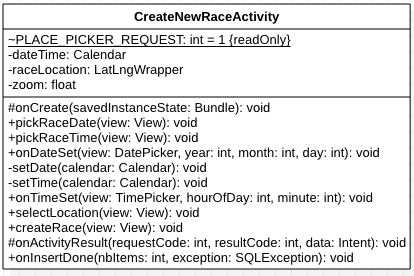
\includegraphics[width=1\columnwidth]{createnewrace_uml.png} 
		\caption{Diagramme de classe}
		\label{fig:createnewrace_uml}
    \end{subfigure}
    ~ %add desired spacing between images, e. g. ~, \quad, \qquad, \hfill etc. 
      %(or a blank line to force the subfigure onto a new line)
    \begin{subfigure}[htb]{0.49\textwidth}
		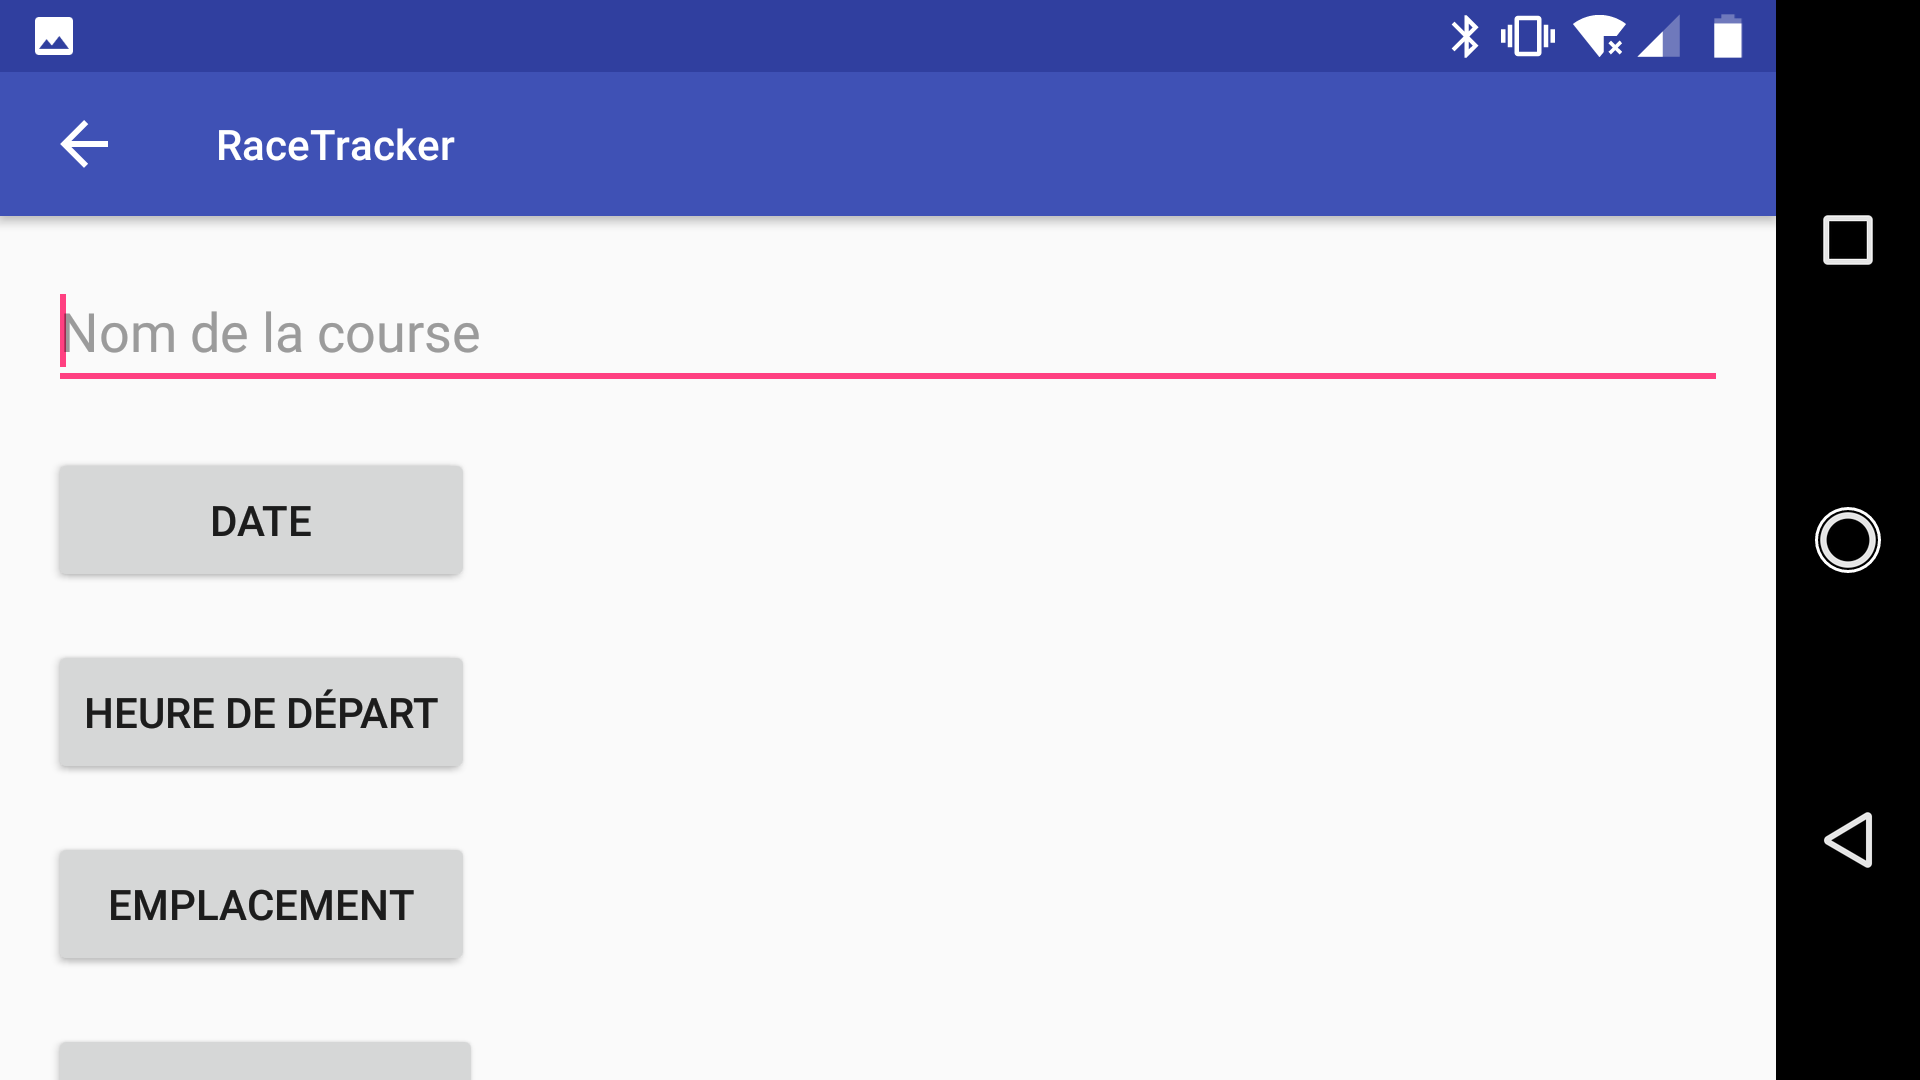
\includegraphics[width=1\columnwidth]{createnewrace_gui.png} 
		\caption{Aperçu de l'interface graphique de l'activité}
		\label{fig:createnewrace_gui}
    \end{subfigure}
    \caption{CreateNewRaceActivity}\label{fig:createnewrace_fig}
\end{figure}

\subsection{RaceLocationPickerActivity}

Permet la sélection de la position où se tient la compétition lors de la création de nouvelles courses. Cette information est utilisée pour pouvoir centrer la vue sur le bon emplacement.

La figure \ref{fig:racelocationpicker_uml} montre le diagramme de classe de RaceLocationPickerActivity.

\begin{figure}[htb!]
    \centering
    \begin{subfigure}[htb]{0.49\textwidth}
		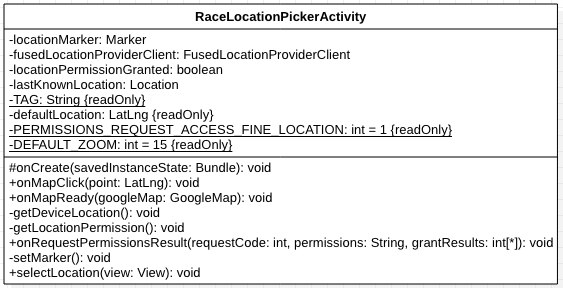
\includegraphics[width=1\columnwidth]{racelocationpicker_uml.png} 
		\caption{Diagramme de classe}
		\label{fig:racelocationpicker_uml}
    \end{subfigure}
    ~ %add desired spacing between images, e. g. ~, \quad, \qquad, \hfill etc. 
      %(or a blank line to force the subfigure onto a new line)
    \begin{subfigure}[htb]{0.49\textwidth}
		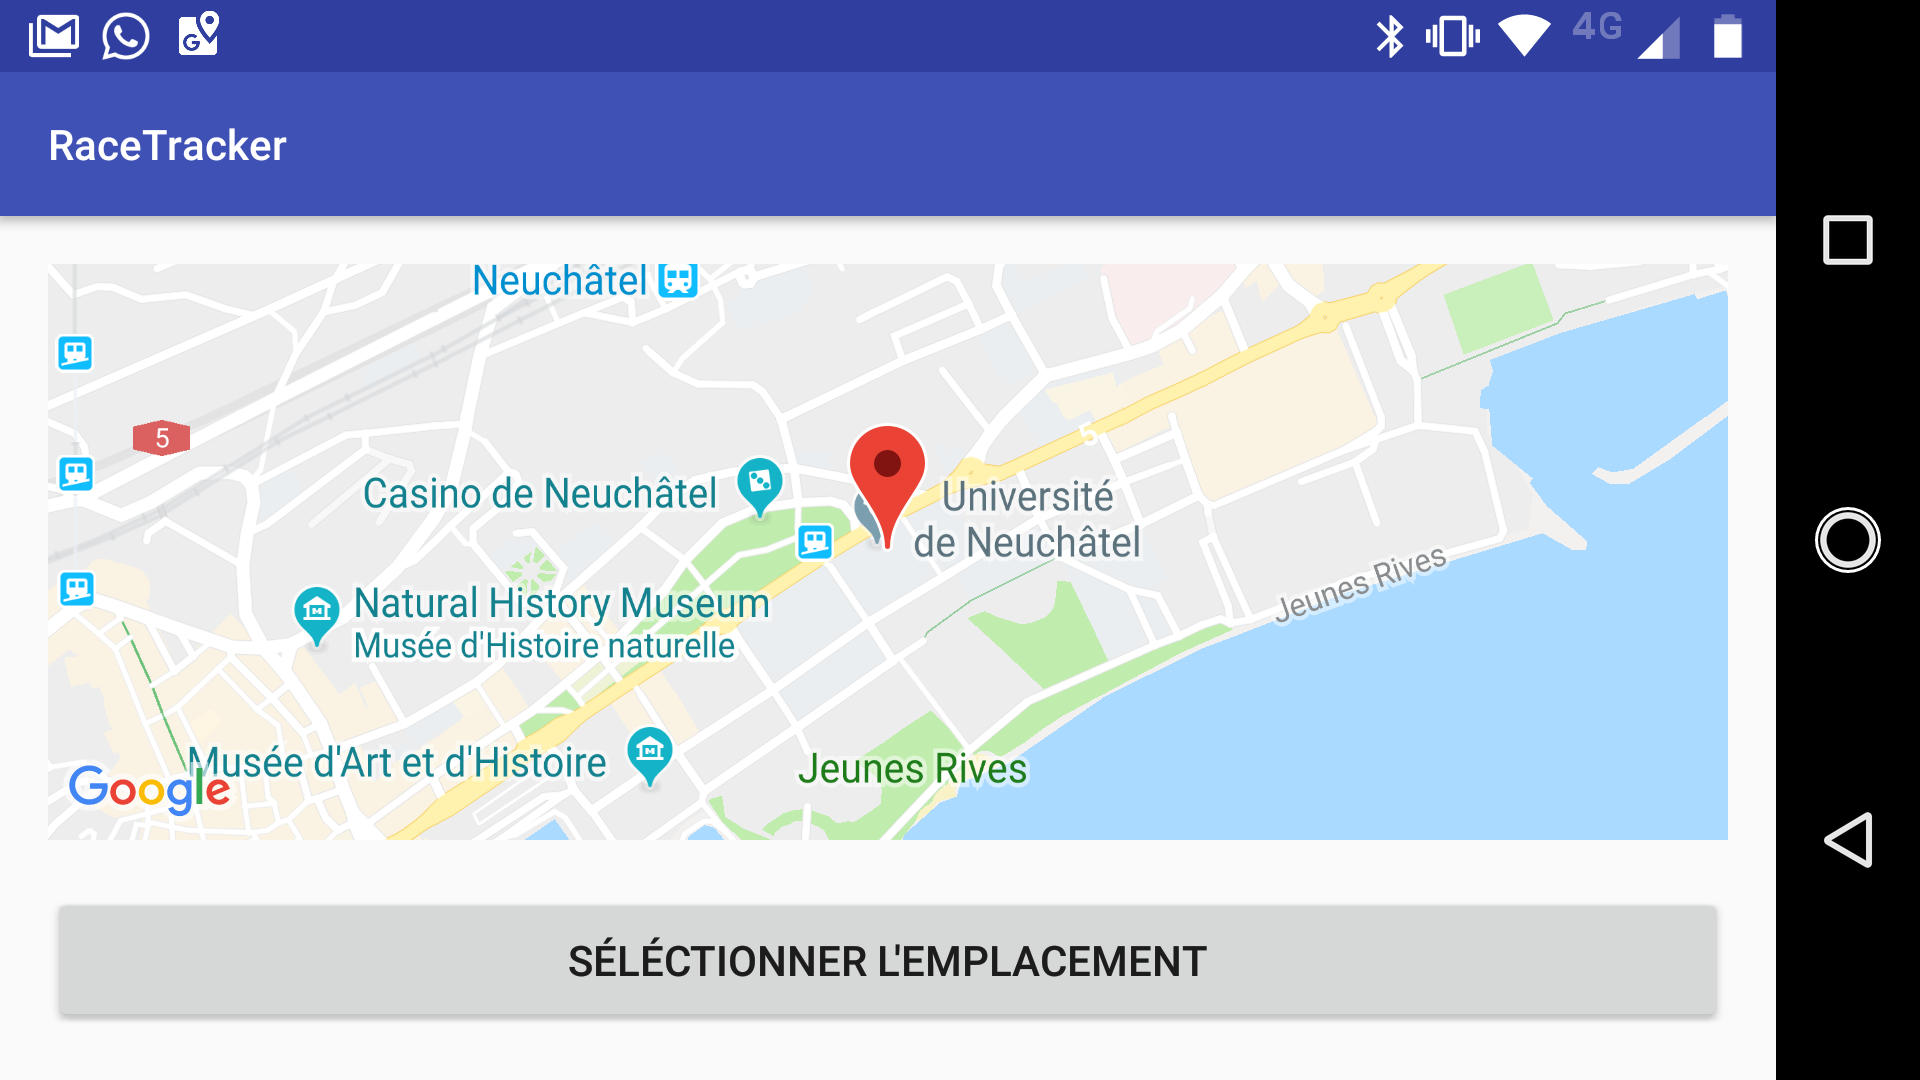
\includegraphics[width=1\columnwidth]{racelocationpicker_gui.png} 
		\caption{Aperçu de l'interface graphique de l'activité}
		\label{fig:racelocationpicker_gui}
    \end{subfigure}
    \caption{RaceLocationPickerActivity}\label{fig:racelocationpicker_fig}
\end{figure}

\subsection{CreateNewCompetitorActivity}

Cette activité permet la création d'un nouveau compétiteur et de son ajout dans la base de données. Une fois rajouté, il pourra ensuite être inscrit à des compétitions.

La figure \ref{fig:createnewcompetitor_uml} montre le diagramme de classe de CreateNewCompetitorActivity.

\begin{figure}[htb!]
    \centering
    \begin{subfigure}[htb]{0.49\textwidth}
		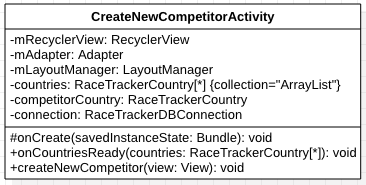
\includegraphics[width=1\columnwidth]{createnewcompetitor_uml.png} 
		\caption{Diagramme de classe}
		\label{fig:createnewcompetitor_uml}
    \end{subfigure}
    ~ %add desired spacing between images, e. g. ~, \quad, \qquad, \hfill etc. 
      %(or a blank line to force the subfigure onto a new line)
    \begin{subfigure}[htb]{0.49\textwidth}
		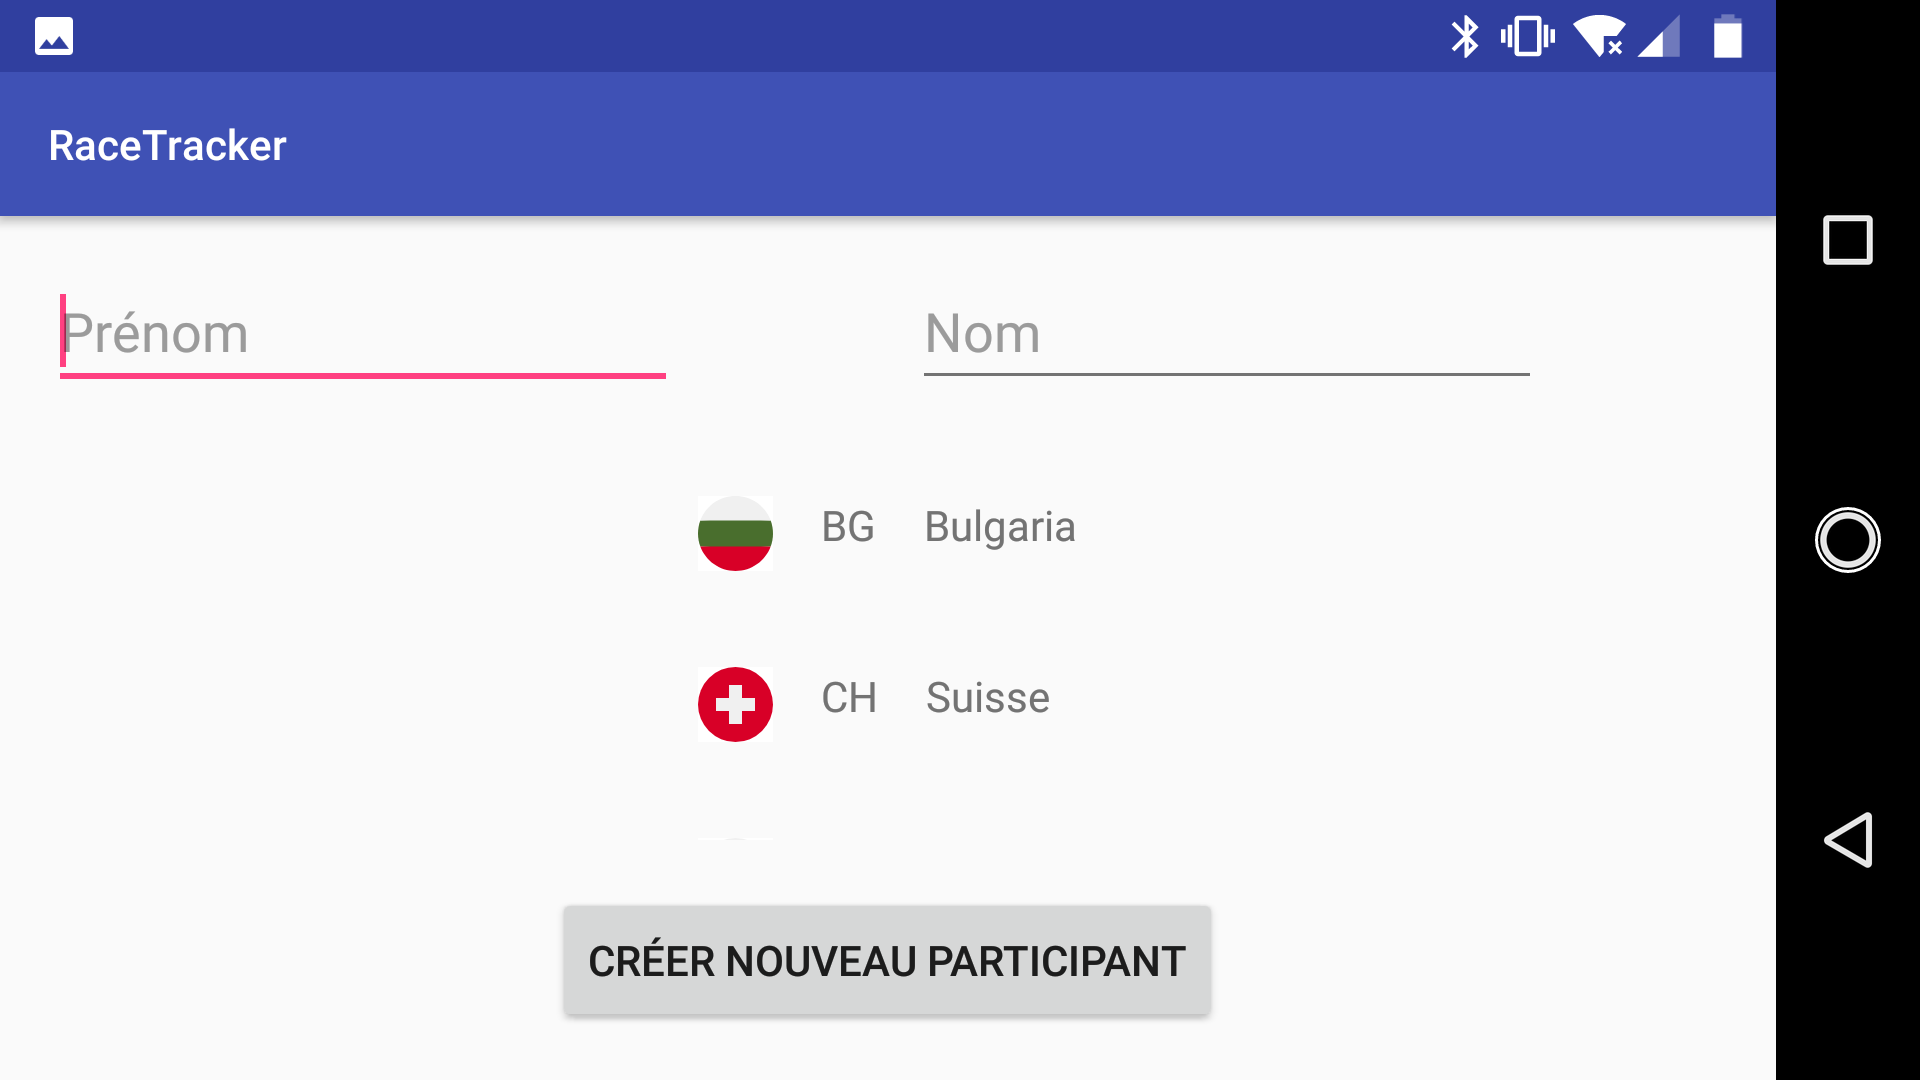
\includegraphics[width=1\columnwidth]{createnewcompetitor_gui.png} 
		\caption{Aperçu de l'interface graphique de l'activité}
		\label{fig:createnewcompetitor_gui}
    \end{subfigure}
    \caption{CreateNewCompetitorActivity}\label{fig:createnewcompetitor_fig}
\end{figure}

\subsection{RegistrationActivity}

Liste les compétiteur déjà inscrits à la compétition sélectionnée. En plus de cela il est possible d'ajouter un nouveau participant, ce qui sera géré par l'activité RegistrationEditActivity.

La figure \ref{fig:registration_uml} montre le diagramme de classe de RegistrationActivity.

\begin{figure}[htb!]
    \centering
    \begin{subfigure}[htb]{0.49\textwidth}
		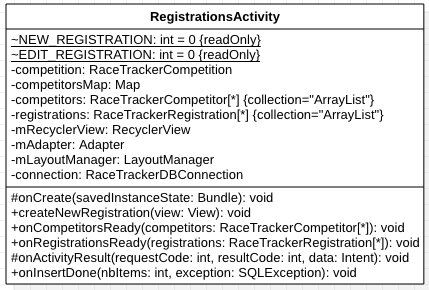
\includegraphics[width=1\columnwidth]{registration_uml.png} 
		\caption{Diagramme de classe}
		\label{fig:registration_uml}
    \end{subfigure}
    ~ %add desired spacing between images, e. g. ~, \quad, \qquad, \hfill etc. 
      %(or a blank line to force the subfigure onto a new line)
    \begin{subfigure}[htb]{0.49\textwidth}
		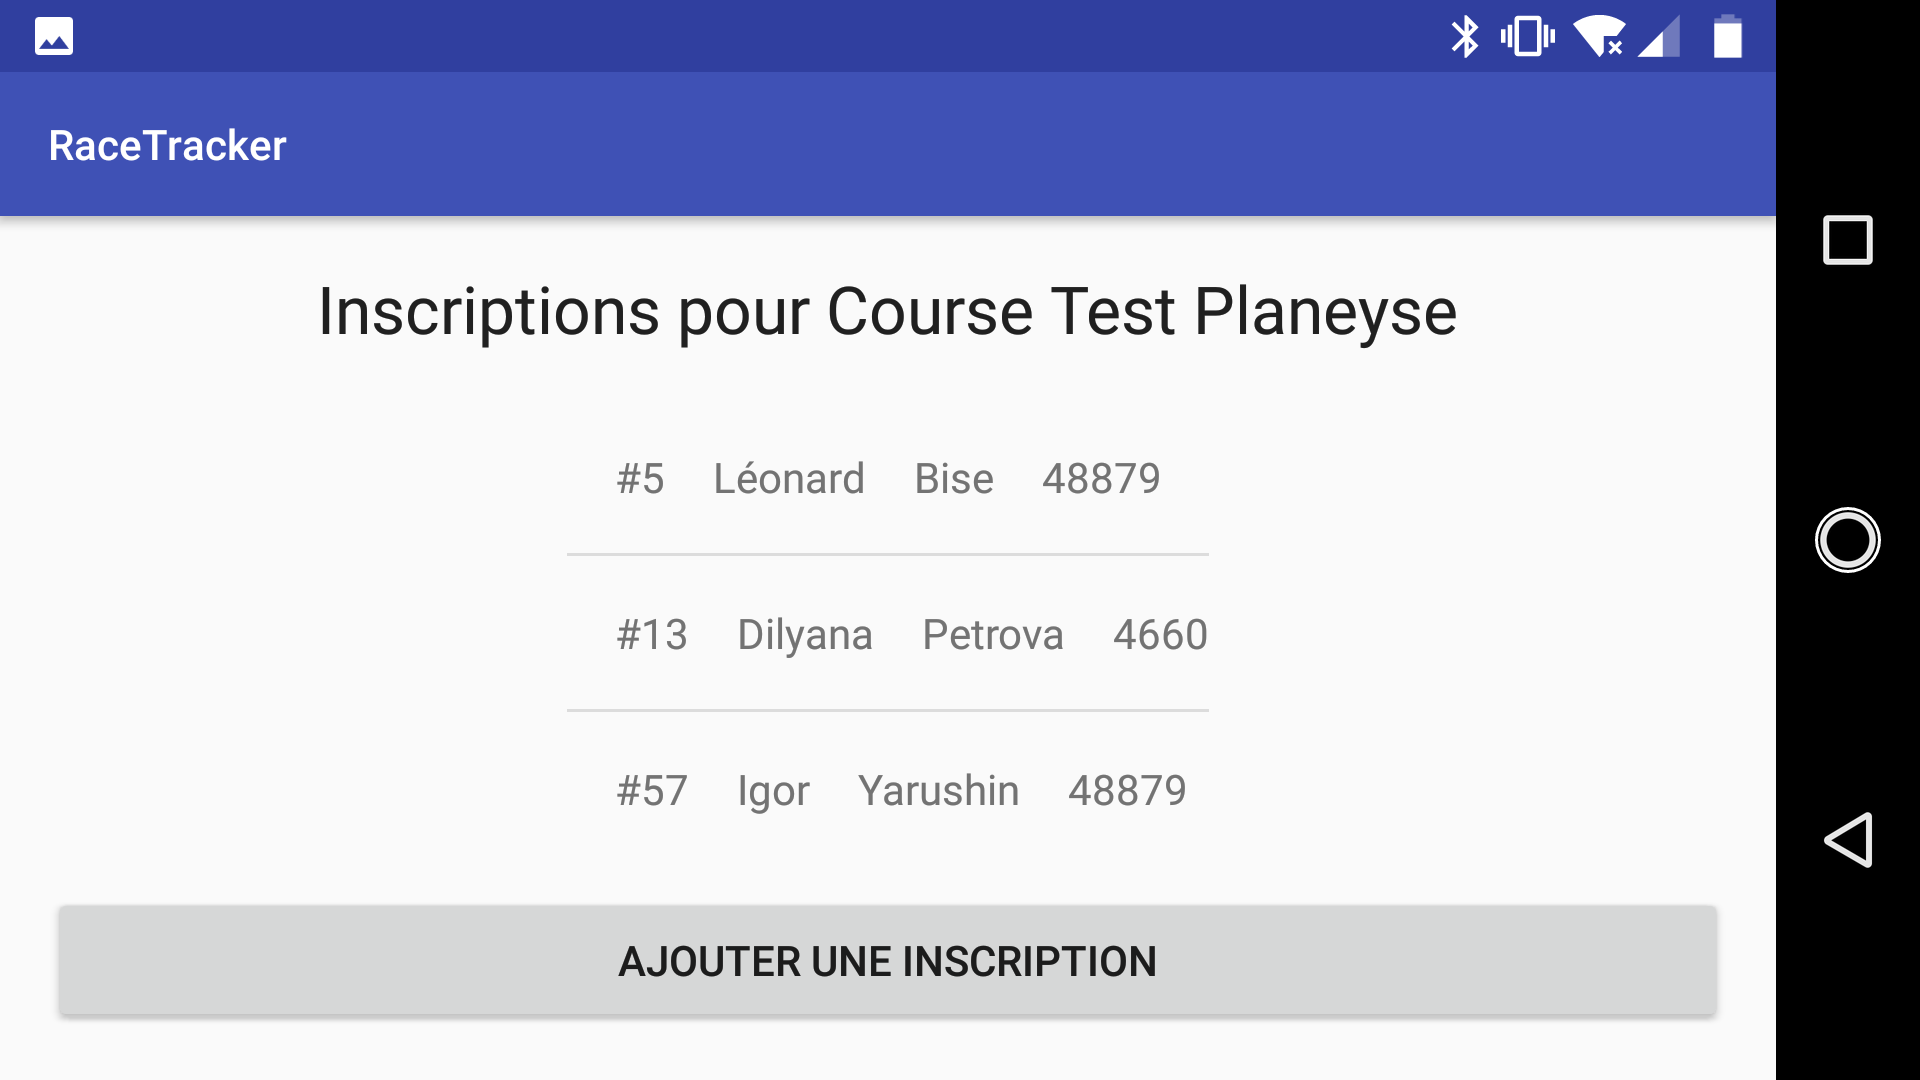
\includegraphics[width=1\columnwidth]{registration_gui.png} 
		\caption{Aperçu de l'interface graphique de l'activité}
		\label{fig:registration_gui}
    \end{subfigure}
    \caption{RegistrationActivity}\label{fig:registration_fig}
\end{figure}

\subsection{RegistrationEditActivity}

Permet l'inscription des concurrents à une certaine course. Un numéro de dossard ainsi que le numéro du capteur qu'ils vont porter durant la course sera également enregistré.

La figure \ref{fig:registrationedit_uml} montre le diagramme de classe de RegistrationEditActivity.

\begin{figure}[htb!]
    \centering
    \begin{subfigure}[htb]{0.49\textwidth}
		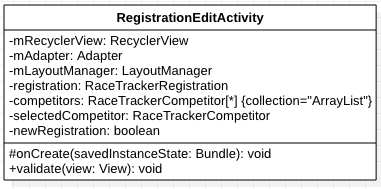
\includegraphics[width=1\columnwidth]{registrationedit_uml.png} 
		\caption{Diagramme de classe}
		\label{fig:registrationedit_uml}
    \end{subfigure}
    ~ %add desired spacing between images, e. g. ~, \quad, \qquad, \hfill etc. 
      %(or a blank line to force the subfigure onto a new line)
    \begin{subfigure}[htb]{0.49\textwidth}
		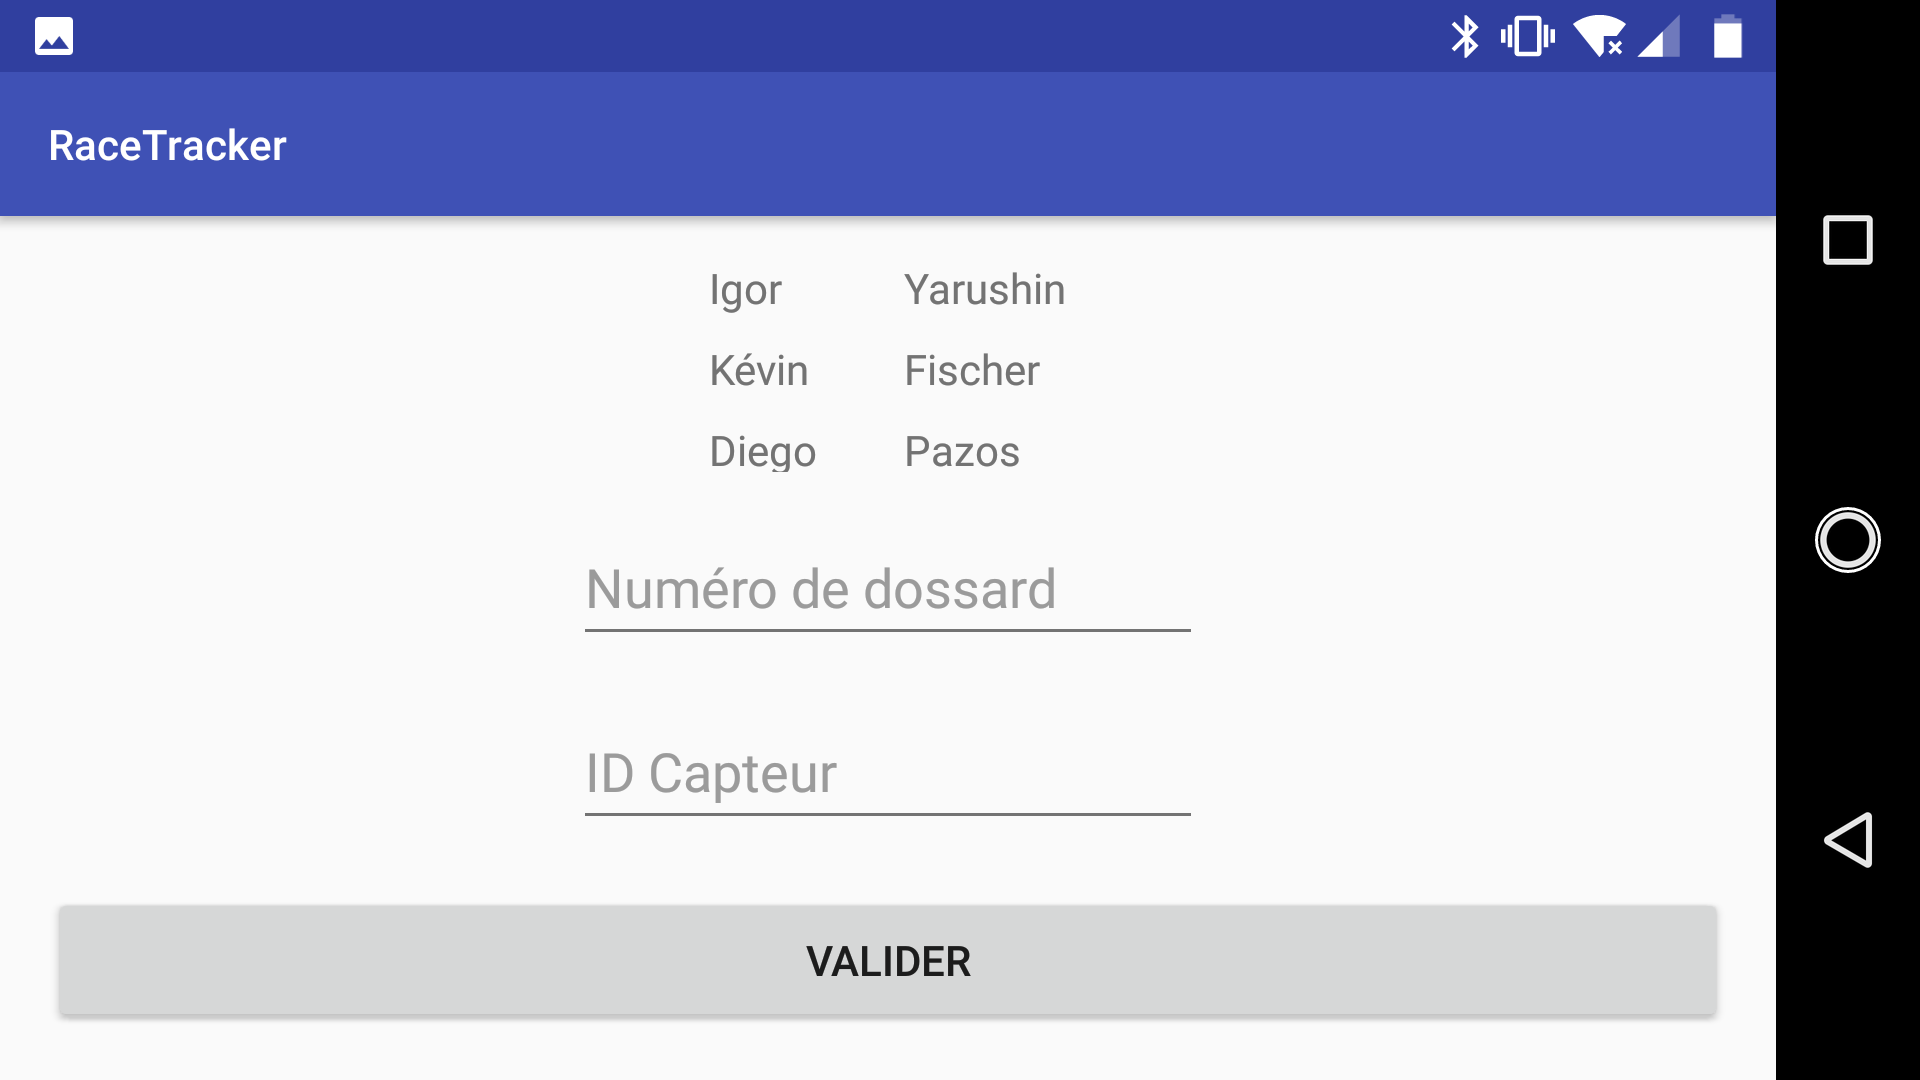
\includegraphics[width=1\columnwidth]{registrationedit_gui.png} 
		\caption{Aperçu de l'interface graphique de l'activité}
		\label{fig:registrationedit_gui}
    \end{subfigure}
    \caption{RegistrationEditActivity}\label{fig:registrationedit_fig}
\end{figure}

\subsection{StartEndRaceActivity}

Cette activité donne la possibilité d'altérer l'état d'une course. Il existe deux états possibles, active ou inactive. Une course active est entrain de se dérouler en direct alors qu'une course inactive est terminée. Dans le cas d'une course en direct, l'activité ViewRaceActivity va alors rechercher les nouveaux points ajoutés à la course et les mettre à jour en temps réel. Pour une course inactive, c'est à dire terminée, c'est une autre activité qui servira à sa visualisation, ReplayRaceActivity. Elle simulera l'affichage des points comme lorsque la course s'est réellement passée, ce qui permet de revoir l'évolution de la compétition.

La figure \ref{fig:startendrace_uml} montre le diagramme de classe de StartEndRaceActivity.

\begin{figure}[htb!]
    \centering
    \begin{subfigure}[htb]{0.49\textwidth}
		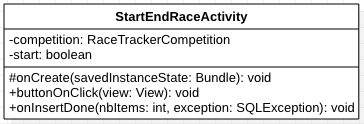
\includegraphics[width=1\columnwidth]{startendrace_uml.png} 
		\caption{Diagramme de classe}
		\label{fig:startendrace_uml}
    \end{subfigure}
    ~ %add desired spacing between images, e. g. ~, \quad, \qquad, \hfill etc. 
      %(or a blank line to force the subfigure onto a new line)
    \begin{subfigure}[htb]{0.49\textwidth}
		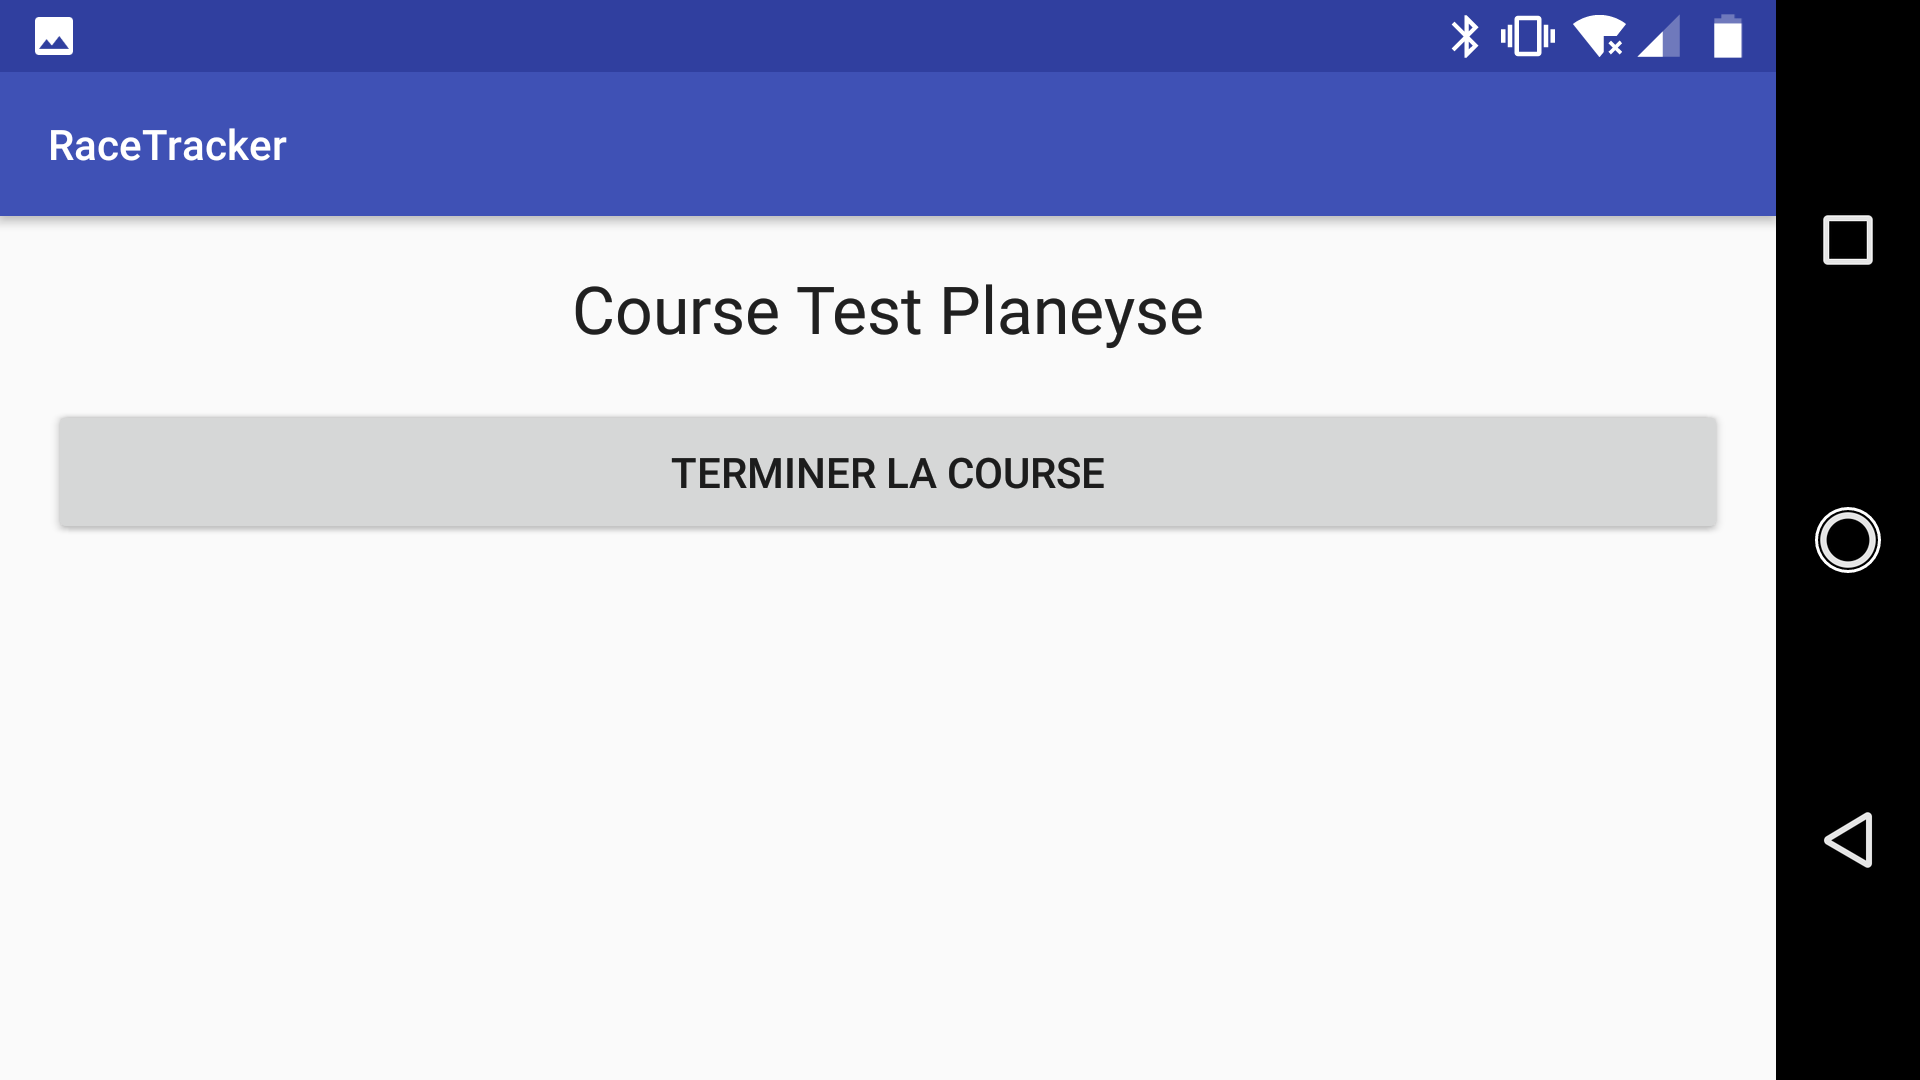
\includegraphics[width=1\columnwidth]{startendrace_gui.png} 
		\caption{Aperçu de l'interface graphique de l'activité}
		\label{fig:startendrace_gui}
    \end{subfigure}
    \caption{StartEndRaceActivity}\label{fig:startendrace_fig}
\end{figure}

\subsection{SettingsActivity}

Cette classe est en charge de la gestion de l'affichage du menu des paramètres. L'utilisateur peut modifier les paramètres relatifs à l'application grâce au menu proposé par cette activité.

La figure \ref{fig:settingsactivity_uml} montre le diagramme de classe de SettingsActivity.

\begin{figure}[htb!]
    \centering
    \begin{subfigure}[htb]{0.49\textwidth}
		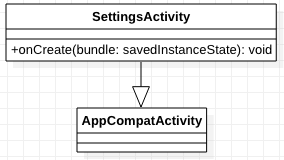
\includegraphics[width=1\columnwidth]{settingsactivity_uml.png} 
		\caption{Diagramme de classe}
		\label{fig:settingsactivity_uml}
    \end{subfigure}
    ~ %add desired spacing between images, e. g. ~, \quad, \qquad, \hfill etc. 
      %(or a blank line to force the subfigure onto a new line)
    \begin{subfigure}[htb]{0.49\textwidth}
		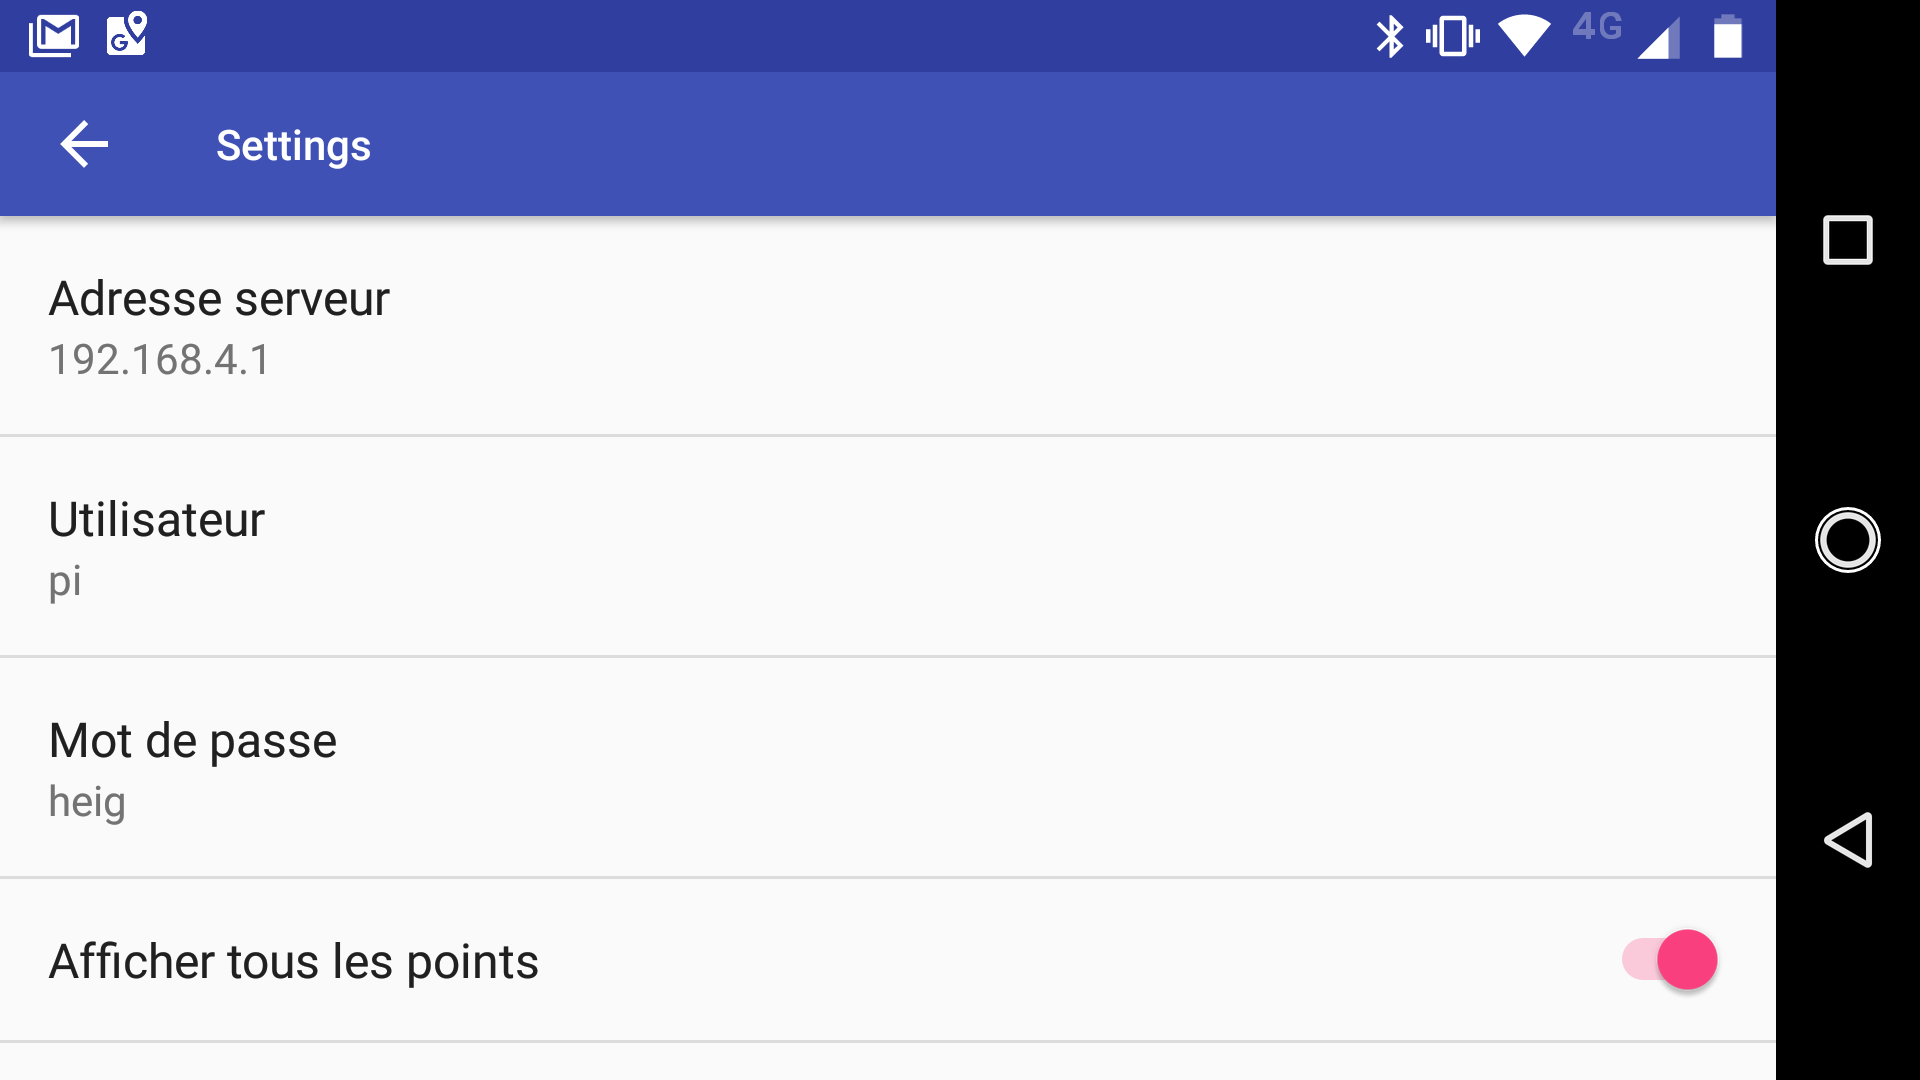
\includegraphics[width=1\columnwidth]{settingsactivity_gui.png} 
		\caption{Aperçu de l'interface graphique de l'activité}
		\label{fig:settingsactivity_gui}
    \end{subfigure}
    \caption{SettingsActivity}\label{fig:settingsactivity_fig}
\end{figure}

\section{Les fragments}

Les fragments représentent le comportement d'une partie de l'interface graphique. Il est possible d'avoir plusieurs fragments sur une même activité.

\subsection{DatePickerFragment}

Le fragment DataPickerFragment est utilisé pour récupérer une date entrée par l'utilisateur, l'interface habituelle pour entrer une date est présentée à l'utilisateur et son choix est retourné.

La figure \ref{fig:datapickerfragment_uml} montre le diagramme de classe de DatePickerFragment.

\begin{figure}[htb!]
    \centering
    \begin{subfigure}[htb]{0.49\textwidth}
		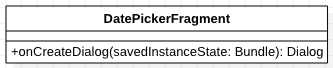
\includegraphics[width=1\columnwidth]{datepickerfragment_uml.png} 
		\caption{Diagramme de classe}
		\label{fig:datepickerfragment_uml}
    \end{subfigure}
    ~ %add desired spacing between images, e. g. ~, \quad, \qquad, \hfill etc. 
      %(or a blank line to force the subfigure onto a new line)
    \begin{subfigure}[htb]{0.49\textwidth}
		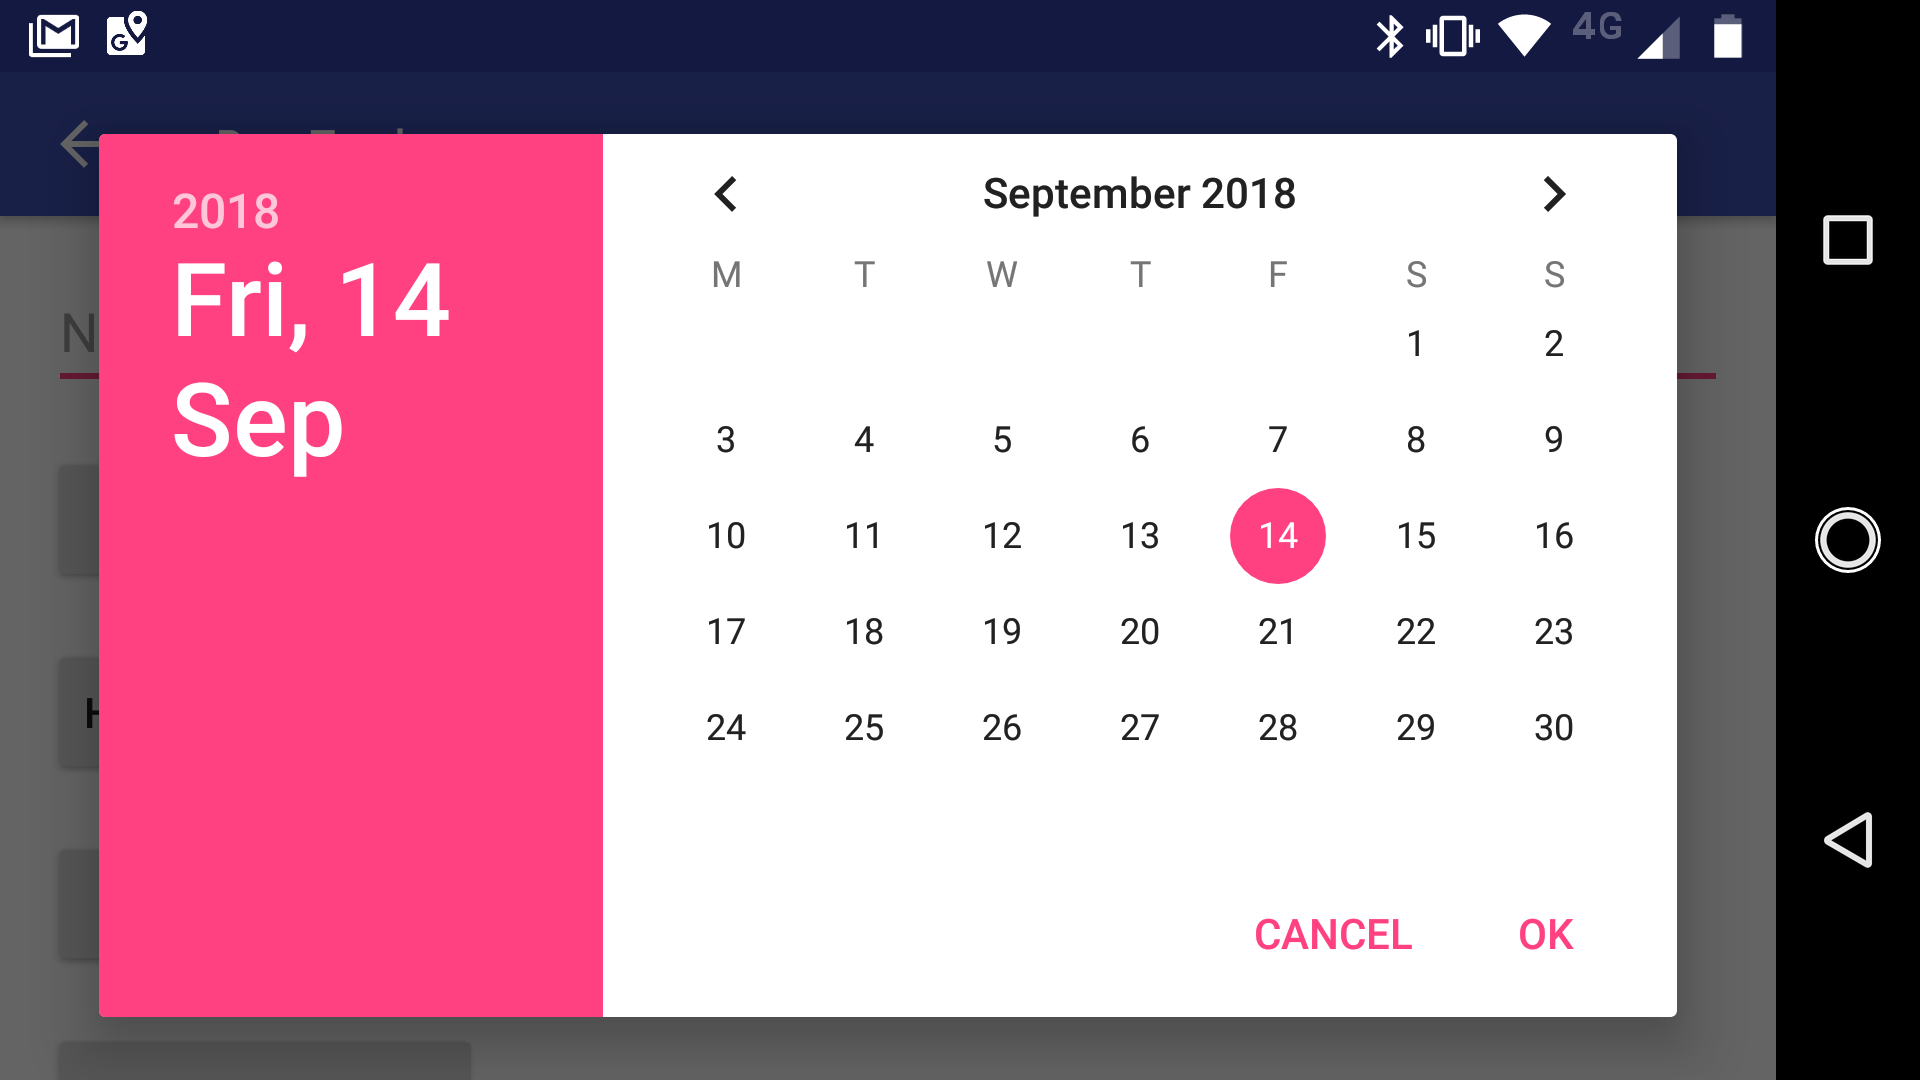
\includegraphics[width=1\columnwidth]{datepickerfragment_gui.png} 
		\caption{Aperçu de l'interface graphique de l'activité}
		\label{fig:datepickerfragment_gui}
    \end{subfigure}
    \caption{DatePickerFragment}\label{fig:datepickerfragment_fig}
\end{figure}

\subsection{TimePickerFragment}

Le fragment TimePickerFragment permet la sélection d'une heure, il présente à l'utilisateur l'interface usuelle de sélection de l'heure puis en retourne le choix.

La figure \ref{fig:timepickerfragment_uml} montre le diagramme de classe de TimePickerFragment.

\begin{figure}[htb!]
    \centering
    \begin{subfigure}[htb]{0.49\textwidth}
		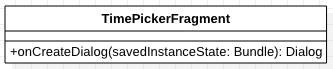
\includegraphics[width=1\columnwidth]{timepickerfragment_uml.png} 
		\caption{Diagramme de classe}
		\label{fig:timepickerfragment_uml}
    \end{subfigure}
    ~ %add desired spacing between images, e. g. ~, \quad, \qquad, \hfill etc. 
      %(or a blank line to force the subfigure onto a new line)
    \begin{subfigure}[htb]{0.49\textwidth}
		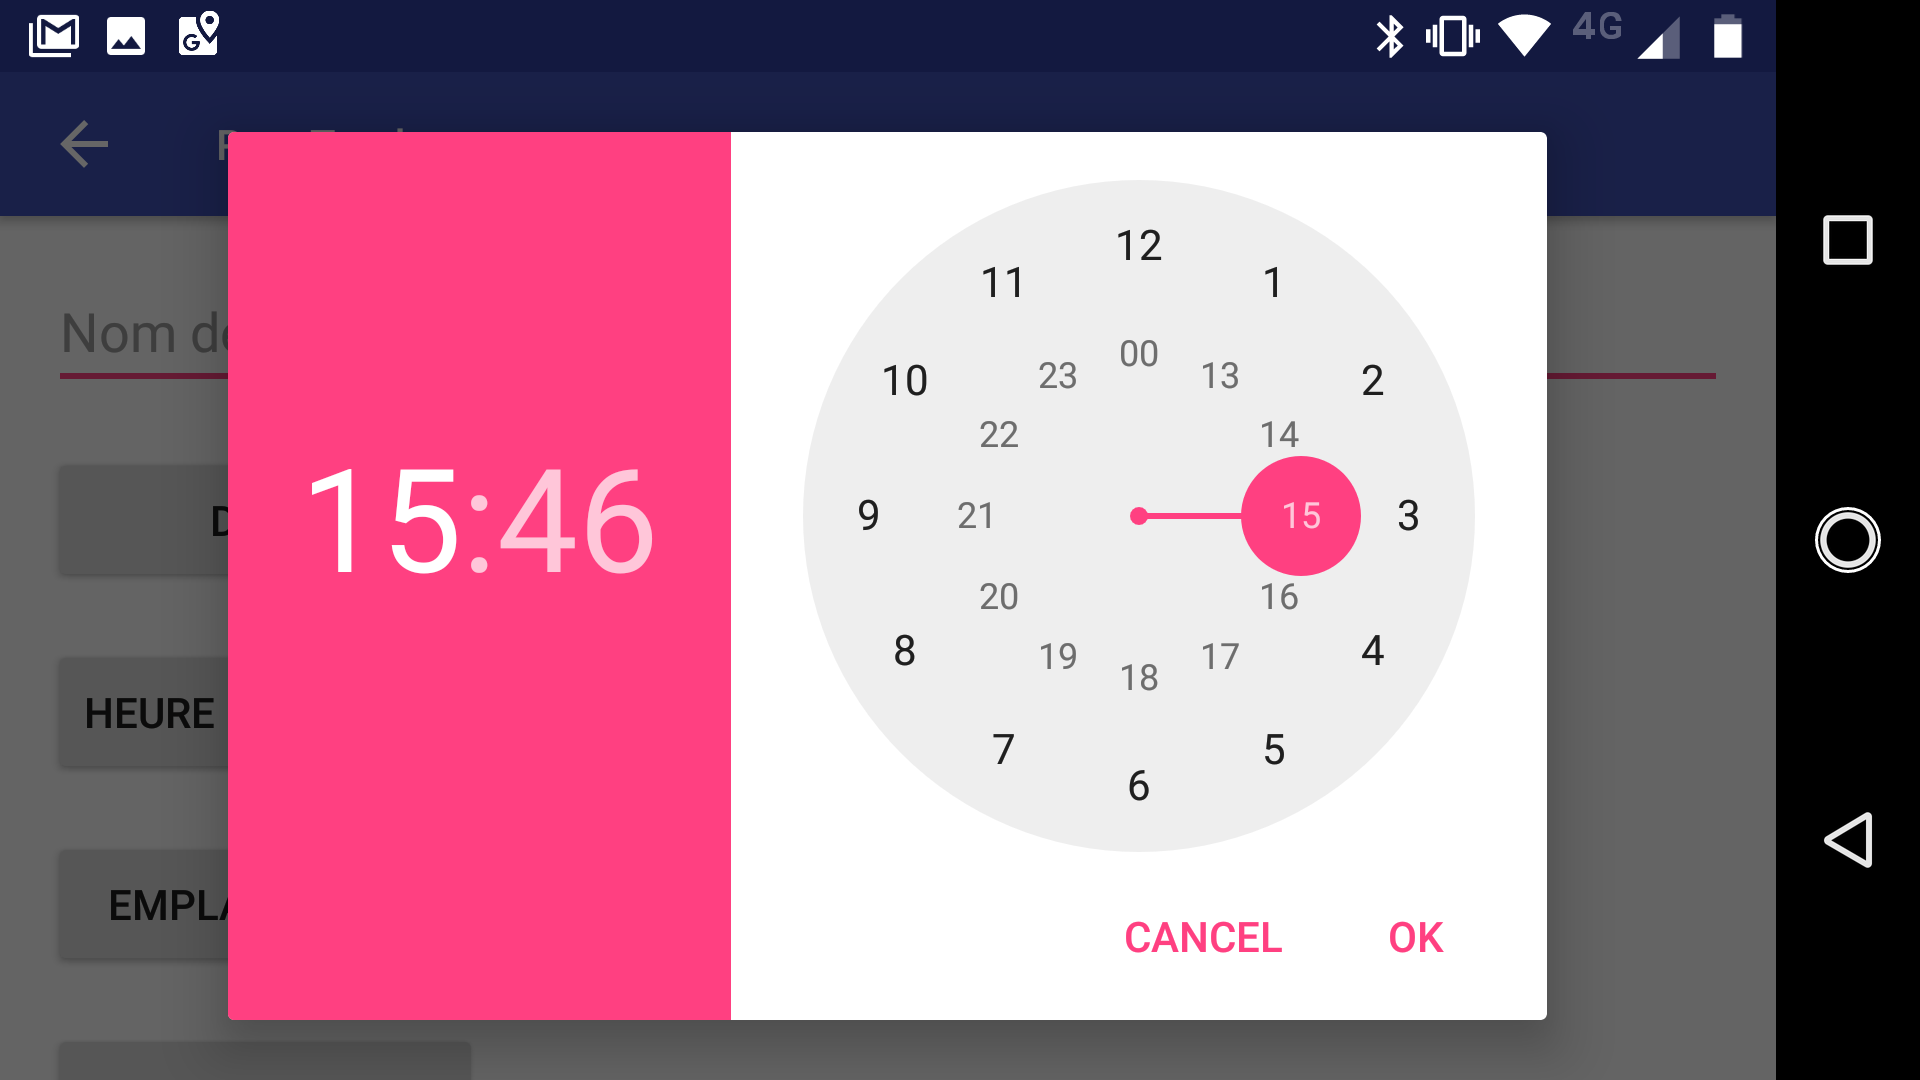
\includegraphics[width=1\columnwidth]{timepickerfragment_gui.png} 
		\caption{Aperçu de l'interface graphique de l'activité}
		\label{fig:timepickerfragment_gui}
    \end{subfigure}
    \caption{TimePickerFragment}\label{fig:timepickerfragment_fig}
\end{figure}

\section{Les classes}

L'application mobile RaceTracker est composée de plusieurs classes qui lui permettent d'effectuer ses différentes tâches. Elles sont décrites dans cette section.

\subsection{RaceTrackerCompetition}

Cette classe contient les données relatives à une compétition. Elle peut être initialisée directement en lui passant le résultat d'une requête à une base de données (ResultSet).

La figure \ref{fig:racetrackercompetition_uml} montre le diagramme de classe de RaceTrackerCompetition.

\begin{figure}[htb!]
    \centering
    \begin{subfigure}[htb]{1\textwidth}
		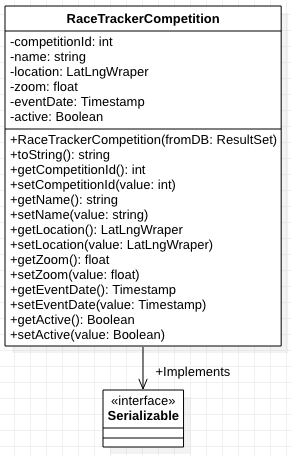
\includegraphics[width=0.5\columnwidth]{racetrackercompetition_uml.png} 
		\caption{Diagramme de classe}
		\label{fig:racetrackercompetition_uml}
    \end{subfigure}
    \begin{subfigure}[htb]{1\textwidth}
		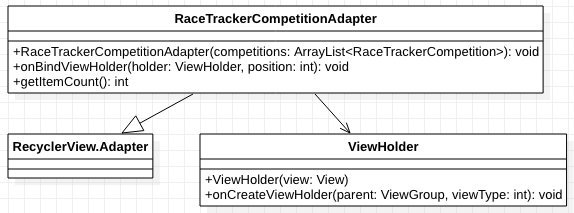
\includegraphics[width=1\columnwidth]{racetrackercompetitionadapter_uml.png} 
		\caption{Diagramme de classe}
		\label{fig:racetrackercompetitionadapter_uml}
    \end{subfigure}
    \begin{subfigure}[htb]{1\textwidth}
		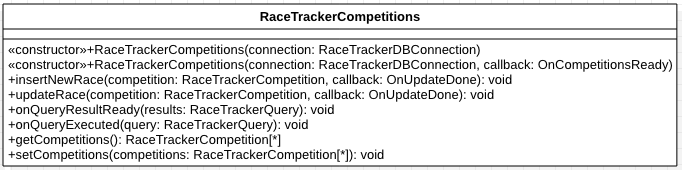
\includegraphics[width=1\columnwidth]{racetrackercompetitions_uml.png} 
		\caption{Diagramme de classe}
		\label{fig:racetrackercompetitions_uml}
    \end{subfigure}
    \caption{RaceTrackerCompetition}\label{fig:racetrackercompetition_fig}
\end{figure}

\subsection{RaceTrackerCompetitionAdapter}

Cette classe permet de faire la gestion de l'affichage d'une liste d'instance de RaceTrackerCompetition dans un objet de type RecyclerView.

La figure \ref{fig:racetrackercompetitionadapter_uml} montre le diagramme de classe de RaceTrackerCompetitionAdapter.

\subsection{RaceTrackerCompetitions}

Cette classe permet de faire le lien avec la base de données. Elle permet de récupérer la liste de toutes les compétitions mais également l'ajout de nouvelles courses ou la modification de courses existantes.

La figure \ref{fig:racetrackercompetitions_uml} montre le diagramme de classe de RaceTrackerCompetitions.

\subsection{RaceTrackerCompetitor}

Cette classe contient les données relatives à un compétiteur. Elle peut être initialisée directement en lui passant le résultat d'une requête à une base de données (ResultSet).

La figure \ref{fig:racetrackercompetitor_uml} montre le diagramme de classe de RaceTrackerCompetitor.

\begin{figure}[htb!]
    \centering
    \begin{subfigure}[htb]{1\textwidth}
		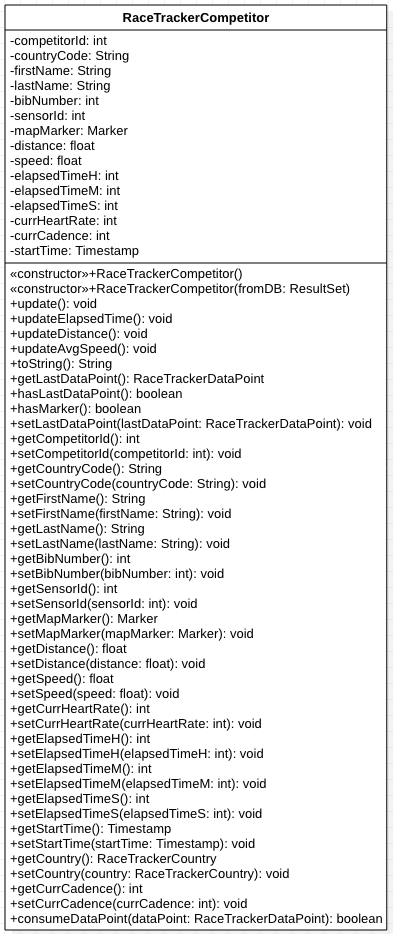
\includegraphics[width=0.5\columnwidth]{racetrackercompetitor_uml.png} 
		\caption{Diagramme de classe}
		\label{fig:racetrackercompetitor_uml}
    \end{subfigure}
    \begin{subfigure}[htb]{1\textwidth}
		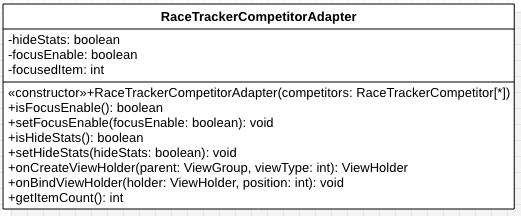
\includegraphics[width=0.7\columnwidth]{racetrackercompetitoradapter_uml.png} 
		\caption{Diagramme de classe}
		\label{fig:racetrackercompetitoradapter_uml}
    \end{subfigure}
    \caption{RaceTrackerCompetitor}\label{fig:racetrackercompetitor_fig}
\end{figure}

\subsection{RaceTrackerCompetitorAdapter}

Cette classe permet de faire la gestion de l'affichage d'une liste d'instance de RaceTrackerCompetitor dans un objet de type RecyclerView.

La figure \ref{fig:racetrackercompetitoradapter_uml} montre le diagramme de classe de RaceTrackerCompetitorAdapter.

\subsection{RaceTrackerCompetitors}

Permet de faire la liaison avec la base de données. Elle permet la récupération de tous les compétiteurs existants dans la base ainsi que l'ajout de nouveaux compétiteurs.

La figure \ref{fig:racetrackercompetitors_uml} montre le diagramme de classe de RaceTrackerCompetitors.

\begin{figure}[htb]
\centering 
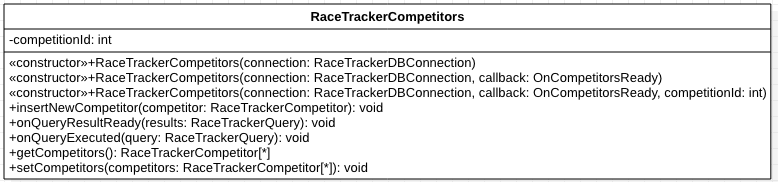
\includegraphics[width=1\columnwidth]{racetrackercompetitors_uml.png} 
\caption{Diagramme de classe de RaceTrackerCompetitors}
\label{fig:racetrackercompetitors_uml}
 \end{figure}

\subsection{RaceTrackerCountry}

Représente un pays dont un compétiteur peut être originaire. Cette classe s'occupe également de la gestion de l'icône du drapeau du pays qui est directement récupéré depuis la base.

La figure \ref{fig:racetrackercountry_uml} montre le diagramme de classe de RaceTrackerCountry.

\begin{figure}[htb!]
    \centering
    \begin{subfigure}[htb]{1\textwidth}
		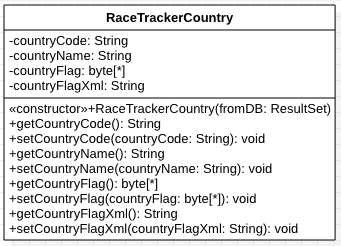
\includegraphics[width=0.5\columnwidth]{racetrackercountry_uml.png} 
		\caption{Diagramme de classe}
		\label{fig:racetrackercountry_uml}
    \end{subfigure}
    \begin{subfigure}[htb]{1\textwidth}
		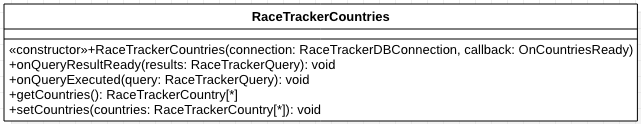
\includegraphics[width=1\columnwidth]{racetrackercountries_uml.png} 
		\caption{Diagramme de classe}
		\label{fig:racetrackercountries_uml}
    \end{subfigure}
    \begin{subfigure}[htb]{1\textwidth}
		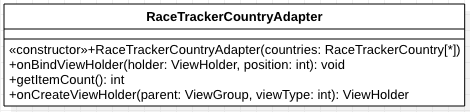
\includegraphics[width=0.8\columnwidth]{racetrackercountryadapter_uml.png} 
		\caption{Diagramme de classe}
		\label{fig:racetrackercountryadapter_uml}
    \end{subfigure}
    \caption{RaceTrackerCountry}\label{fig:racetrackercountry_fig}
\end{figure}

\subsection{RaceTrackerCountryAdapter}

Cette classe permet de faire la gestion de l'affichage d'une liste d'instance de RaceTrackerCountry dans un objet de type RecyclerView.

La figure \ref{fig:racetrackercountryadapter_uml} montre le diagramme de classe de RaceTrackerCountryAdapter.

\subsection{RaceTrackerCountries}

Permet la gestion de la liste de tous les pays qu'elle récupère directement depuis la base de données.

La figure \ref{fig:racetrackercountries_uml} montre le diagramme de classe de RaceTrackerCountries.

\subsection{RaceTrackerRegistration}

La classe RaceTrackerRegistration contient les information relative à une inscription à une course spécifique.

La figure \ref{fig:racetrackerregistration_uml} montre le diagramme de classe de RaceTrackerRegistration.

\begin{figure}[htb!]
    \centering
    \begin{subfigure}[htb]{1\textwidth}
		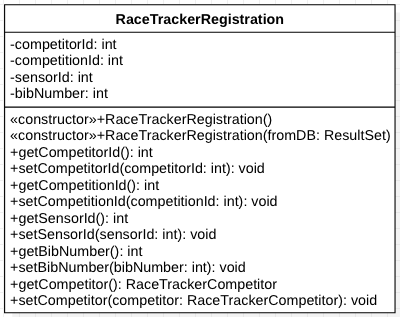
\includegraphics[width=0.5\columnwidth]{racetrackerregistration_uml.png} 
		\caption{Diagramme de classe}
		\label{fig:racetrackerregistration_uml}
    \end{subfigure}
    \begin{subfigure}[htb]{1\textwidth}
		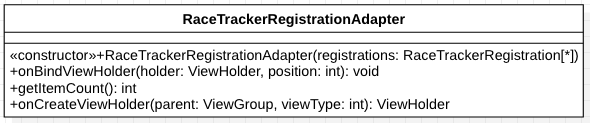
\includegraphics[width=0.8\columnwidth]{racetrackerregistrationadapter_uml.png} 
		\caption{Diagramme de classe}
		\label{fig:racetrackerregistrationadapter_uml}
    \end{subfigure}
    \begin{subfigure}[htb]{1\textwidth}
		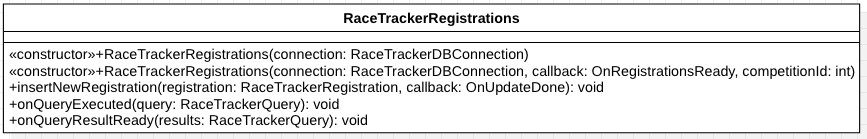
\includegraphics[width=1\columnwidth]{racetrackerregistrations_uml.png} 
		\caption{Diagramme de classe}
		\label{fig:racetrackerregistrations_uml}
    \end{subfigure}
    \caption{RaceTrackerRegistration}\label{fig:racetrackerregistration_fig}
\end{figure}

\subsection{RaceTrackerRegistrationAdapter}

Cette classe permet de faire la gestion de l'affichage d'une liste d'instance de RaceTrackerRegistration dans un objet de type RecyclerView.

La figure \ref{fig:racetrackerregistrationadapter_uml} montre le diagramme de classe de RaceTrackerRegistrationAdapter.

\subsection{RaceTrackerRegistrations}

Permet la récupération d'une liste de RaceTrackerRegistration pour une certaine course depuis la base de données. C'est également cette classe qui permet l'insertion de nouvelles inscriptions.

La figure \ref{fig:racetrackerregistrations_uml} montre le diagramme de classe de RaceTrackerRegistrations.

\subsection{RaceTrackerDataPoint}

La classe RaceTrackerDataPoint contient les données relatives à un point de données sur le parcours. C'est ce type de classe que le ViewRaceActivity utilise afin d'afficher à l'utilisateur la position et les informations associées aux coureurs. Elle peut être initialisée directement en lui passant le résultat d'une requête à une base de donnée (ResultSet). Chaque data point correspond à un paquet de donnée envoyé par le capteur et contient toutes les données qui étaient parties de la charge utile du paquet.

La figure \ref{fig:racetrackerdatapoint_uml} montre le diagramme de classe de RaceTrackerDataPoint.
 
 \begin{figure}[htb!]
    \centering
    \begin{subfigure}[htb]{1\textwidth}
		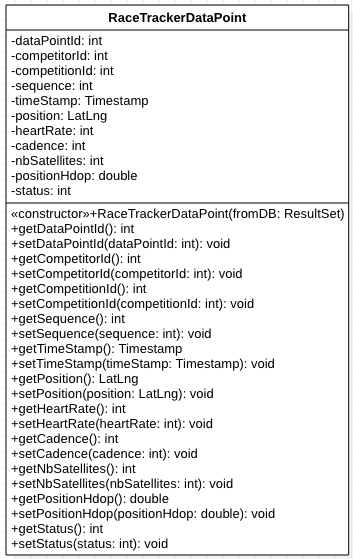
\includegraphics[width=0.5\columnwidth]{racetrackerdatapoint_uml.png} 
		\caption{Diagramme de classe}
		\label{fig:racetrackerdatapoint_uml}
    \end{subfigure}
    \begin{subfigure}[htb]{1\textwidth}
		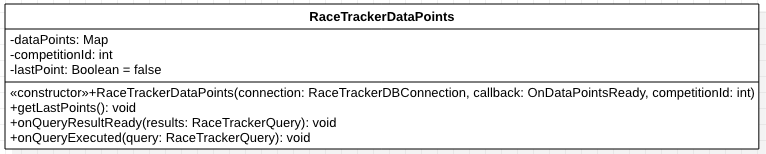
\includegraphics[width=1\columnwidth]{racetrackerdatapoints_uml.png} 
		\caption{Diagramme de classe}
		\label{fig:racetrackerdatapoints_uml}
    \end{subfigure}
    \caption{RaceTrackerDataPoint}\label{fig:racetrackerdatapoints_fig}
\end{figure}

\subsection{RaceTrackerDataPoints}

Permet de récupérer une liste de RaceTrackerDataPoint initialisée directement depuis les données reçues depuis la base de données.

La figure \ref{fig:racetrackerdatapoints_uml} montre le diagramme de classe de RaceTrackerDataPoints.

\subsection{RaceTrackerTrackPoint}

Les track points représentent toutes les positions qui sont utilisées pour pouvoir dessiner le tracé du parcours de la course. Ils sont stockés dans la base de données et il est possible de les lire grâce à la classe RaceTrackerTrackPoints.

La figure \ref{fig:racetrackertrackpoint_uml} montre le diagramme de classe de RaceTrackerTrackPoint.
 
 \begin{figure}[htb!]
    \centering
    \begin{subfigure}[htb]{1\textwidth}
		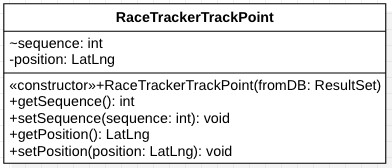
\includegraphics[width=0.5\columnwidth]{racetrackertrackpoint_uml.png} 
		\caption{Diagramme de classe}
		\label{fig:racetrackertrackpoint_uml}
    \end{subfigure}
    \begin{subfigure}[htb]{1\textwidth}
		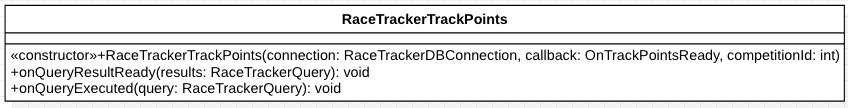
\includegraphics[width=1\columnwidth]{racetrackertrackpoints_uml.png} 
		\caption{Diagramme de classe}
		\label{fig:racetrackertrackpoints_uml}
    \end{subfigure}
    \caption{RaceTrackerTrackPoint}\label{fig:racetrackertrackpoint_fig}
\end{figure}

\subsection{RaceTrackerTrackPoints}

Cette classe permet la récupération de tous les points du parcours de la course depuis la base de données. Ils sont ensuite passés à la carte Google map afin d'y dessiner le parcours.

La figure \ref{fig:racetrackertrackpoints_uml} montre le diagramme de classe de RaceTrackerTrackPoints.

\subsection{RaceTrackerDBConnection}

La classe qui contient les informations relatives à la connexion à la base de données, c'est à dire adresse, user name et mots de passe. Elle permet ensuite de construire la chaîne de caractères utilisée par le driver JDBC.

La figure \ref{fig:racetrackercompetitors_uml} montre le diagramme de classe de RaceTrackerCompetitors.

\begin{figure}[htb]
\centering 
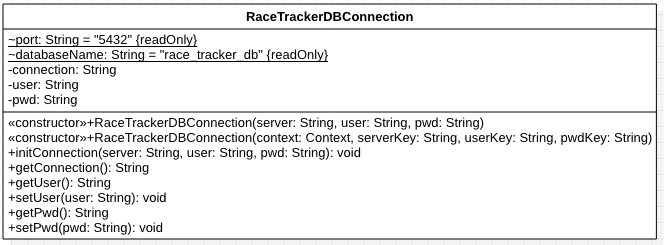
\includegraphics[width=1\columnwidth]{racetrackerdbconnection_uml.png} 
\caption{Diagramme de classe de RaceTrackerDBConnection}
\label{fig:racetrackerdbconnection_uml}
 \end{figure}

\subsection{RaceTrackerQuery}

Contient une requête pour la base de donnée, son résultat, la fonction de callback de l'utilisateur et éventuellement l'exception si la requête n'a pas pu être exécutée correctement. Cette classe permet d'exécuter deux types de requêtes, les requêtes dites de mise à jour (DELETE, UPDATE ou INSERT) ou de sélection (SELECT).

Deux types de fonction callback sont utilisées pour informer l'utilisateur de l'évolution de la requête. OnQueryResultReady est déclenché lorsque les résultats d'une sélection sont prêts à être analysés. OnQueryExecuted est déclenché au terme de l'opération de sélection ou de mise à jour.

La figure \ref{fig:racetrackerquery_uml} montre le diagramme de classe de RaceTrackerQuery.

 \begin{figure}[htb]
    \centering
    \begin{subfigure}[htb]{1\textwidth}
		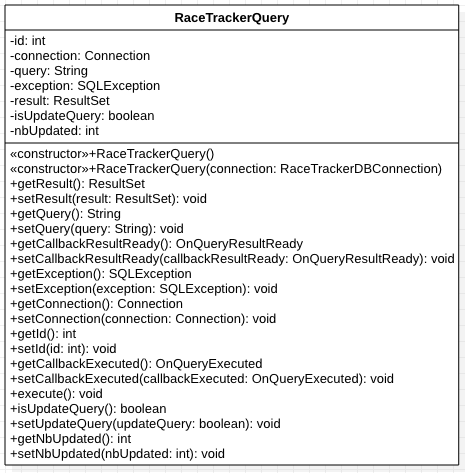
\includegraphics[width=0.7\columnwidth]{racetrackerquery_uml.png} 
		\caption{Diagramme de classe}
		\label{fig:racetrackerquery_uml}
    \end{subfigure}
    \begin{subfigure}[htb]{1\textwidth}
		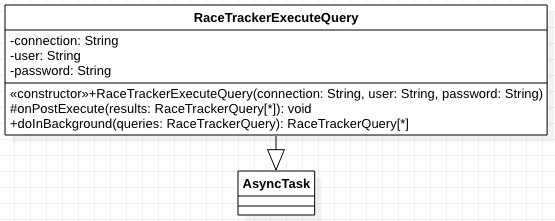
\includegraphics[width=0.9\columnwidth]{racetrackerexecutequery_uml.png} 
		\caption{Diagramme de classe}
		\label{fig:racetrackerexecutequery_uml}
    \end{subfigure}
        \begin{subfigure}[htb]{1\textwidth}
		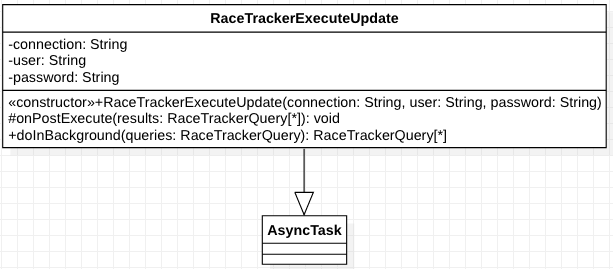
\includegraphics[width=0.9\columnwidth]{racetrackerexecuteupdate_uml.png} 
		\caption{Diagramme de classe}
		\label{fig:racetrackerexecuteupdate_uml}
    \end{subfigure}
    \caption{RaceTrackerQuery}\label{fig:racetrackerquery_fig}
\end{figure}

\subsection{RaceTrackerExecuteQuery}

Cette classe, qui hérite de AsyncTask, permet l'exécution d'une requête RaceTrackerQuery de type mise à jour de manière asynchrone dans le but de ne pas bloquer le thread principal d'affichage d'Android.

La figure \ref{fig:racetrackerexecutequery_uml} montre le diagramme de classe de RaceTrackerExecuteQuery.

\subsection{RaceTrackerExecuteUpdate}

Cette classe, qui hérite de AsyncTask permet l'exécution d'une requête RaceTrackerQuery de type sélection de manière asynchrone dans le but de ne pas bloquer le thread principal d'affichage d'Android.

La figure \ref{fig:racetrackerexecutequery_uml} montre le diagramme de classe de RaceTrackerExecuteUpdate.

\subsection{LatLngWraper}

Cette classe permet d'encapsuler un objet de type LatLng. Cette classe est utilisée pour rendre un objet LatLng serialisable.

La figure \ref{fig:latlngwraper_uml} montre le diagramme de classe de LatLngWraper.

\begin{figure}[htb]
\centering 
\includegraphics[width=0.4\columnwidth]{latlngwraper_uml.png} 
\caption{Diagramme de classe de LatLngWraper}
\label{fig:latlngwraper_uml}
 \end{figure}

\subsection{RecyclerTouchListener}

Cette classe permet de faciliter la gestion des événements OnClick des RecyclerView.

La figure \ref{fig:recyclertouchlistener_uml} montre le diagramme de classe de RecyclerTouchListener.

\begin{figure}[htb]
\centering 
\includegraphics[width=1\columnwidth]{recyclertouchlistener_uml.png} 
\caption{Diagramme de classe de RecyclerTouchListener}
\label{fig:recyclertouchlistener_uml}
 \end{figure}

\section{Les interfaces}

\subsection{OnQueryResultReady}

OnQueryResultReady est une interface que l'utilisateur doit implémenter afin de pouvoir recevoir les résultats des requêtes envoyées à la base de données. La fonction est automatiquement appelée lorsque les résultats de la requête associée sont prêts à être consultés. Cette interface est appelée depuis le contexte d'exécution de AsyncTask, c'est à dire en arrière-plan (et non sur le thread d'affichage de l'UI, ce qui ne permet donc pas d'interagir avec les éléments graphiques lors de son appel).

La figure \ref{fig:onqueryresultready_uml} montre le diagramme de classe de OnQueryResultReady.

\begin{figure}[htb]
\centering 
\includegraphics[width=0.6\columnwidth]{onqueryresultready_uml.png} 
\caption{Diagramme de classe de OnQueryResultReady}
\label{fig:onqueryresultready_uml}
 \end{figure}

\subsection{OnQueryExecuted}

Cette interface permet à l'utilisateur de savoir lorsque l'exécution d'une requête est terminée. L'interface OnQueryExecuted est appelée depuis le contexte d'exécution du thread d'affichage de l'UI et donc permet à l'utilisateur de modifier des éléments d'affichage ou de remplir des listes de type RecyclerView.

La figure \ref{fig:onqueryexecuted_uml} montre le diagramme de classe de OnQueryExecuted.

\begin{figure}[htb]
\centering 
\includegraphics[width=0.6\columnwidth]{onqueryexecuted_uml.png} 
\caption{Diagramme de classe de OnQueryExecuted}
\label{fig:onqueryexecuted_uml}
 \end{figure}

\subsection{OnUpdateDone}

OnUpdateDone est appelé au terme de l'exécution d'une requête de type mise à jour. Elle permet de connaître le nombre d'éléments qui ont été mis à jour ainsi que l'éventuelle exception qui serait survenue durant son exécution.

La figure \ref{fig:onupdatedone_uml} montre le diagramme de classe de OnUpdateDone.

\begin{figure}[htb]
\centering 
\includegraphics[width=0.7\columnwidth]{onupdatedone_uml.png} 
\caption{Diagramme de classe de OnUpdateDone}
\label{fig:onupdatedone_uml}
 \end{figure}
